\documentclass[]{book}
\usepackage{lmodern}
\usepackage{amssymb,amsmath}
\usepackage{ifxetex,ifluatex}
\usepackage{fixltx2e} % provides \textsubscript
\ifnum 0\ifxetex 1\fi\ifluatex 1\fi=0 % if pdftex
  \usepackage[T1]{fontenc}
  \usepackage[utf8]{inputenc}
\else % if luatex or xelatex
  \ifxetex
    \usepackage{mathspec}
  \else
    \usepackage{fontspec}
  \fi
  \defaultfontfeatures{Ligatures=TeX,Scale=MatchLowercase}
\fi
% use upquote if available, for straight quotes in verbatim environments
\IfFileExists{upquote.sty}{\usepackage{upquote}}{}
% use microtype if available
\IfFileExists{microtype.sty}{%
\usepackage{microtype}
\UseMicrotypeSet[protrusion]{basicmath} % disable protrusion for tt fonts
}{}
\usepackage[margin=1in]{geometry}
\usepackage{hyperref}
\hypersetup{unicode=true,
            pdftitle={MEM52220 - Applied Econometrics},
            pdfauthor={Nicolas Reigl},
            pdfborder={0 0 0},
            breaklinks=true}
\urlstyle{same}  % don't use monospace font for urls
\usepackage{natbib}
\bibliographystyle{apalike}
\usepackage{color}
\usepackage{fancyvrb}
\newcommand{\VerbBar}{|}
\newcommand{\VERB}{\Verb[commandchars=\\\{\}]}
\DefineVerbatimEnvironment{Highlighting}{Verbatim}{commandchars=\\\{\}}
% Add ',fontsize=\small' for more characters per line
\usepackage{framed}
\definecolor{shadecolor}{RGB}{248,248,248}
\newenvironment{Shaded}{\begin{snugshade}}{\end{snugshade}}
\newcommand{\AlertTok}[1]{\textcolor[rgb]{0.94,0.16,0.16}{#1}}
\newcommand{\AnnotationTok}[1]{\textcolor[rgb]{0.56,0.35,0.01}{\textbf{\textit{#1}}}}
\newcommand{\AttributeTok}[1]{\textcolor[rgb]{0.77,0.63,0.00}{#1}}
\newcommand{\BaseNTok}[1]{\textcolor[rgb]{0.00,0.00,0.81}{#1}}
\newcommand{\BuiltInTok}[1]{#1}
\newcommand{\CharTok}[1]{\textcolor[rgb]{0.31,0.60,0.02}{#1}}
\newcommand{\CommentTok}[1]{\textcolor[rgb]{0.56,0.35,0.01}{\textit{#1}}}
\newcommand{\CommentVarTok}[1]{\textcolor[rgb]{0.56,0.35,0.01}{\textbf{\textit{#1}}}}
\newcommand{\ConstantTok}[1]{\textcolor[rgb]{0.00,0.00,0.00}{#1}}
\newcommand{\ControlFlowTok}[1]{\textcolor[rgb]{0.13,0.29,0.53}{\textbf{#1}}}
\newcommand{\DataTypeTok}[1]{\textcolor[rgb]{0.13,0.29,0.53}{#1}}
\newcommand{\DecValTok}[1]{\textcolor[rgb]{0.00,0.00,0.81}{#1}}
\newcommand{\DocumentationTok}[1]{\textcolor[rgb]{0.56,0.35,0.01}{\textbf{\textit{#1}}}}
\newcommand{\ErrorTok}[1]{\textcolor[rgb]{0.64,0.00,0.00}{\textbf{#1}}}
\newcommand{\ExtensionTok}[1]{#1}
\newcommand{\FloatTok}[1]{\textcolor[rgb]{0.00,0.00,0.81}{#1}}
\newcommand{\FunctionTok}[1]{\textcolor[rgb]{0.00,0.00,0.00}{#1}}
\newcommand{\ImportTok}[1]{#1}
\newcommand{\InformationTok}[1]{\textcolor[rgb]{0.56,0.35,0.01}{\textbf{\textit{#1}}}}
\newcommand{\KeywordTok}[1]{\textcolor[rgb]{0.13,0.29,0.53}{\textbf{#1}}}
\newcommand{\NormalTok}[1]{#1}
\newcommand{\OperatorTok}[1]{\textcolor[rgb]{0.81,0.36,0.00}{\textbf{#1}}}
\newcommand{\OtherTok}[1]{\textcolor[rgb]{0.56,0.35,0.01}{#1}}
\newcommand{\PreprocessorTok}[1]{\textcolor[rgb]{0.56,0.35,0.01}{\textit{#1}}}
\newcommand{\RegionMarkerTok}[1]{#1}
\newcommand{\SpecialCharTok}[1]{\textcolor[rgb]{0.00,0.00,0.00}{#1}}
\newcommand{\SpecialStringTok}[1]{\textcolor[rgb]{0.31,0.60,0.02}{#1}}
\newcommand{\StringTok}[1]{\textcolor[rgb]{0.31,0.60,0.02}{#1}}
\newcommand{\VariableTok}[1]{\textcolor[rgb]{0.00,0.00,0.00}{#1}}
\newcommand{\VerbatimStringTok}[1]{\textcolor[rgb]{0.31,0.60,0.02}{#1}}
\newcommand{\WarningTok}[1]{\textcolor[rgb]{0.56,0.35,0.01}{\textbf{\textit{#1}}}}
\usepackage{longtable,booktabs}
\usepackage{graphicx,grffile}
\makeatletter
\def\maxwidth{\ifdim\Gin@nat@width>\linewidth\linewidth\else\Gin@nat@width\fi}
\def\maxheight{\ifdim\Gin@nat@height>\textheight\textheight\else\Gin@nat@height\fi}
\makeatother
% Scale images if necessary, so that they will not overflow the page
% margins by default, and it is still possible to overwrite the defaults
% using explicit options in \includegraphics[width, height, ...]{}
\setkeys{Gin}{width=\maxwidth,height=\maxheight,keepaspectratio}
\IfFileExists{parskip.sty}{%
\usepackage{parskip}
}{% else
\setlength{\parindent}{0pt}
\setlength{\parskip}{6pt plus 2pt minus 1pt}
}
\setlength{\emergencystretch}{3em}  % prevent overfull lines
\providecommand{\tightlist}{%
  \setlength{\itemsep}{0pt}\setlength{\parskip}{0pt}}
\setcounter{secnumdepth}{5}
% Redefines (sub)paragraphs to behave more like sections
\ifx\paragraph\undefined\else
\let\oldparagraph\paragraph
\renewcommand{\paragraph}[1]{\oldparagraph{#1}\mbox{}}
\fi
\ifx\subparagraph\undefined\else
\let\oldsubparagraph\subparagraph
\renewcommand{\subparagraph}[1]{\oldsubparagraph{#1}\mbox{}}
\fi

%%% Use protect on footnotes to avoid problems with footnotes in titles
\let\rmarkdownfootnote\footnote%
\def\footnote{\protect\rmarkdownfootnote}

%%% Change title format to be more compact
\usepackage{titling}

% Create subtitle command for use in maketitle
\newcommand{\subtitle}[1]{
  \posttitle{
    \begin{center}\large#1\end{center}
    }
}

\setlength{\droptitle}{-2em}

  \title{MEM52220 - Applied Econometrics}
    \pretitle{\vspace{\droptitle}\centering\huge}
  \posttitle{\par}
    \author{Nicolas Reigl}
    \preauthor{\centering\large\emph}
  \postauthor{\par}
      \predate{\centering\large\emph}
  \postdate{\par}
    \date{2018-07-26}

\usepackage{booktabs}

\begin{document}
\maketitle

{
\setcounter{tocdepth}{1}
\tableofcontents
}
\hypertarget{introduction}{%
\chapter{Introduction}\label{introduction}}

Welcome to MEM5220 - Applied Econometrics. This handout was originally
(and currently) designed for the use with MEM5220 - Applied Econometrics
at Tallinn University of Technology. Note that this workbook is still
under heavy development!

\hypertarget{prerequisites}{%
\section{Prerequisites}\label{prerequisites}}

A basic knowledge of the R \citep{team2013r} programming language is
required.

\hypertarget{resources}{%
\section{Resources}\label{resources}}

Our primary resource is \citet{heiss2016using} \footnote{Heiss (2016)
  builds on the popular Introductory Econometrics by Wooldridge (2016)
  and demonstrates how to replicate the applications discussed therein
  using R.} . For theoretical concepts see
\citet{wooldridge2015introductory}.

\hypertarget{acknowledgements}{%
\section{Acknowledgements}\label{acknowledgements}}

I thank Kadri Männasoo and Juan Carlos Cuestas for proofreading and
their useful comments.

\hypertarget{linearregression}{%
\chapter{Linear Regression}\label{linearregression}}

The general form in which we specify regression models in R:

\begin{Shaded}
\begin{Highlighting}[]
\CommentTok{## response ~ terms}
\CommentTok{## }
\CommentTok{## y ~ age + sex            # age + sex main effects}
\CommentTok{## y ~ age + sex + age:sex  # add second-order interaction}
\CommentTok{## y ~ age*sex              # second-order interaction +}
\CommentTok{##                          # all main effects}
\CommentTok{## y ~ (age + sex + pressure)^2}
\CommentTok{##                          # age+sex+pressure+age:sex+age:pressure...}
\CommentTok{## y ~ (age + sex + pressure)^2 - sex:pressure}
\CommentTok{##                          # all main effects and all 2nd order}
\CommentTok{##                          # interactions except sex:pressure}
\CommentTok{## y ~ (age + race)*sex     # age+race+sex+age:sex+race:sex}
\CommentTok{## y ~ treatment*(age*race + age*sex) # no interact. with race,sex}
\CommentTok{## sqrt(y) ~ sex*sqrt(age) + race}
\CommentTok{## # functions, with dummy variables generated if}
\CommentTok{## # race is an R factor (classification) variable}
\CommentTok{## y ~ sex + poly(age,2)    # poly generates orthogonal polynomials}
\CommentTok{## race.sex <- interaction(race,sex)}
\CommentTok{## y ~ age + race.sex       # for when you want dummy variables for}
\CommentTok{##                          # all combinations of the factors}
\end{Highlighting}
\end{Shaded}

\hypertarget{simple-linear-regression}{%
\section{Simple Linear Regression}\label{simple-linear-regression}}

We start off with a simple OLS Regression. We will work with multiple
data sources:

\begin{itemize}
\tightlist
\item
  Data from \citet{wooldridge2015introductory} : Introductory
  Econometrics: A Modern Approch.
\item
  \emph{More datasources in the future}
\end{itemize}

To load the dataset and necessary functions:

\begin{Shaded}
\begin{Highlighting}[]
\CommentTok{# This function 1. checks if the packages are installed. 2. It installs the packages if they were not in the list of installed packages. 3. It loads the packages into the workspace}
\NormalTok{PACKAGES<-}\KeywordTok{c}\NormalTok{(}\StringTok{"wooldridge"}\NormalTok{,  }\CommentTok{# Wooldrige Datasets}
            \StringTok{"tidyverse"}\NormalTok{,  }\CommentTok{# for data manipulation and ggplots}
            \StringTok{"broom"}\NormalTok{,  }\CommentTok{# Tidy regression output}
            \StringTok{"ggpubr"}\NormalTok{,  }\CommentTok{# Multiple ggplots on a page. Note that, the installation of ggpubr will automatically install the gridExtra and the cowplot package; so you don’t need to re-install them. }
            \StringTok{"ggfortify"}\NormalTok{) }\CommentTok{# Simple ggplot recipe for lm objects)}
\NormalTok{inst<-}\KeywordTok{match}\NormalTok{(PACKAGES, }\KeywordTok{.packages}\NormalTok{(}\DataTypeTok{all=}\OtherTok{TRUE}\NormalTok{))}
\NormalTok{need<-}\KeywordTok{which}\NormalTok{(}\KeywordTok{is.na}\NormalTok{(inst))}
\ControlFlowTok{if}\NormalTok{ (}\KeywordTok{length}\NormalTok{(need)}\OperatorTok{>}\DecValTok{0}\NormalTok{) }\KeywordTok{install.packages}\NormalTok{(PACKAGES[need])}
\KeywordTok{lapply}\NormalTok{(PACKAGES, require, }\DataTypeTok{character.only=}\NormalTok{T)}
\end{Highlighting}
\end{Shaded}

Classic examples of quantities modeled with simple linear regression:

\begin{itemize}
\tightlist
\item
  College GPA ∼ SAT scores \(\beta > 0\)
\item
  Change in GDP ∼ change in unemployment \(\beta < 0\)
\item
  House price ∼ number of bedrooms \(\beta > 0\)
\item
  Species heart weight ∼ species body weight \(\beta > 0\)
\item
  Fatalities per year ∼ speed limit \(\beta < 0\)
\end{itemize}

Notice that these simple linear regressions are simplifications of more
complex relationships between the variables in question.

In this exercise we use the dataset \emph{ceosal1}. Let us analyse the
dataset first

\begin{Shaded}
\begin{Highlighting}[]
\KeywordTok{data}\NormalTok{(}\StringTok{"ceosal1"}\NormalTok{)}
\KeywordTok{help}\NormalTok{(}\StringTok{"ceosal1"}\NormalTok{)}
\NormalTok{?ceosal1}
\end{Highlighting}
\end{Shaded}

As we see from the R documentation the \emph{ceosal1} dataset contain of
a random sample of data reported in the May 6, 1991 issue of
Businessweek.

To get a first look at the data you can use the \texttt{View()} function
inside R Studio.

\begin{Shaded}
\begin{Highlighting}[]
\KeywordTok{View}\NormalTok{(ceosal1)}
\end{Highlighting}
\end{Shaded}

We could also take a look at the variable names, the dimension of the
data frame, and some sample observations with \texttt{str()}.

\begin{Shaded}
\begin{Highlighting}[]
\KeywordTok{str}\NormalTok{(ceosal1)}
\end{Highlighting}
\end{Shaded}

\begin{verbatim}
## 'data.frame':    209 obs. of  12 variables:
##  $ salary  : int  1095 1001 1122 578 1368 1145 1078 1094 1237 833 ...
##  $ pcsalary: int  20 32 9 -9 7 5 10 7 16 5 ...
##  $ sales   : num  27595 9958 6126 16246 21783 ...
##  $ roe     : num  14.1 10.9 23.5 5.9 13.8 ...
##  $ pcroe   : num  106.4 -30.6 -16.3 -25.7 -3 ...
##  $ ros     : int  191 13 14 -21 56 55 62 44 37 37 ...
##  $ indus   : int  1 1 1 1 1 1 1 1 1 1 ...
##  $ finance : int  0 0 0 0 0 0 0 0 0 0 ...
##  $ consprod: int  0 0 0 0 0 0 0 0 0 0 ...
##  $ utility : int  0 0 0 0 0 0 0 0 0 0 ...
##  $ lsalary : num  7 6.91 7.02 6.36 7.22 ...
##  $ lsales  : num  10.23 9.21 8.72 9.7 9.99 ...
##  - attr(*, "time.stamp")= chr "25 Jun 2011 23:03"
\end{verbatim}

As we have seen before in the general R tutorial, there are a number of
additional functions to access some of this information directly.

\begin{Shaded}
\begin{Highlighting}[]
\KeywordTok{dim}\NormalTok{(ceosal1)}
\end{Highlighting}
\end{Shaded}

\begin{verbatim}
## [1] 209  12
\end{verbatim}

\begin{Shaded}
\begin{Highlighting}[]
\KeywordTok{nrow}\NormalTok{(ceosal1)}
\end{Highlighting}
\end{Shaded}

\begin{verbatim}
## [1] 209
\end{verbatim}

\begin{Shaded}
\begin{Highlighting}[]
\KeywordTok{ncol}\NormalTok{(ceosal1)}
\end{Highlighting}
\end{Shaded}

\begin{verbatim}
## [1] 12
\end{verbatim}

\begin{Shaded}
\begin{Highlighting}[]
\KeywordTok{summary}\NormalTok{(ceosal1)}
\end{Highlighting}
\end{Shaded}

\begin{verbatim}
##      salary         pcsalary          sales              roe       
##  Min.   :  223   Min.   :-61.00   Min.   :  175.2   Min.   : 0.50  
##  1st Qu.:  736   1st Qu.: -1.00   1st Qu.: 2210.3   1st Qu.:12.40  
##  Median : 1039   Median :  9.00   Median : 3705.2   Median :15.50  
##  Mean   : 1281   Mean   : 13.28   Mean   : 6923.8   Mean   :17.18  
##  3rd Qu.: 1407   3rd Qu.: 20.00   3rd Qu.: 7177.0   3rd Qu.:20.00  
##  Max.   :14822   Max.   :212.00   Max.   :97649.9   Max.   :56.30  
##      pcroe            ros            indus           finance      
##  Min.   :-98.9   Min.   :-58.0   Min.   :0.0000   Min.   :0.0000  
##  1st Qu.:-21.2   1st Qu.: 21.0   1st Qu.:0.0000   1st Qu.:0.0000  
##  Median : -3.0   Median : 52.0   Median :0.0000   Median :0.0000  
##  Mean   : 10.8   Mean   : 61.8   Mean   :0.3206   Mean   :0.2201  
##  3rd Qu.: 19.5   3rd Qu.: 81.0   3rd Qu.:1.0000   3rd Qu.:0.0000  
##  Max.   :977.0   Max.   :418.0   Max.   :1.0000   Max.   :1.0000  
##     consprod         utility          lsalary          lsales      
##  Min.   :0.0000   Min.   :0.0000   Min.   :5.407   Min.   : 5.166  
##  1st Qu.:0.0000   1st Qu.:0.0000   1st Qu.:6.601   1st Qu.: 7.701  
##  Median :0.0000   Median :0.0000   Median :6.946   Median : 8.217  
##  Mean   :0.2871   Mean   :0.1722   Mean   :6.950   Mean   : 8.292  
##  3rd Qu.:1.0000   3rd Qu.:0.0000   3rd Qu.:7.249   3rd Qu.: 8.879  
##  Max.   :1.0000   Max.   :1.0000   Max.   :9.604   Max.   :11.489
\end{verbatim}

The interesting task here is to determine how far a high the CEO salary
is, for a given return on equity.

\begin{center}\rule{0.5\linewidth}{\linethickness}\end{center}

\textbf{Your turn}

What sign would be expect of \(\beta\) (the slope)?

A: Without seeing the data \textbf{my} prior is that \(\beta > 0\).

\begin{center}\rule{0.5\linewidth}{\linethickness}\end{center}

\textbf{Note}

A simple linear model as assumes that the mean of each \(y_{i}\)
conditioned on \(x_{i}\) is a linear function of \(x_{i}\). But notice
that simple linear regressions are simplifications of more complex
relationships between the variables in question.

\begin{center}\rule{0.5\linewidth}{\linethickness}\end{center}

\begin{Shaded}
\begin{Highlighting}[]
\CommentTok{# Use ggplot style}
\KeywordTok{ggplot}\NormalTok{(ceosal1, }\KeywordTok{aes}\NormalTok{(}\DataTypeTok{x =}\NormalTok{ roe, }\DataTypeTok{y =}\NormalTok{ salary)) }\OperatorTok{+}
\StringTok{  }\KeywordTok{geom_point}\NormalTok{()}
\end{Highlighting}
\end{Shaded}

\begin{figure}
\centering
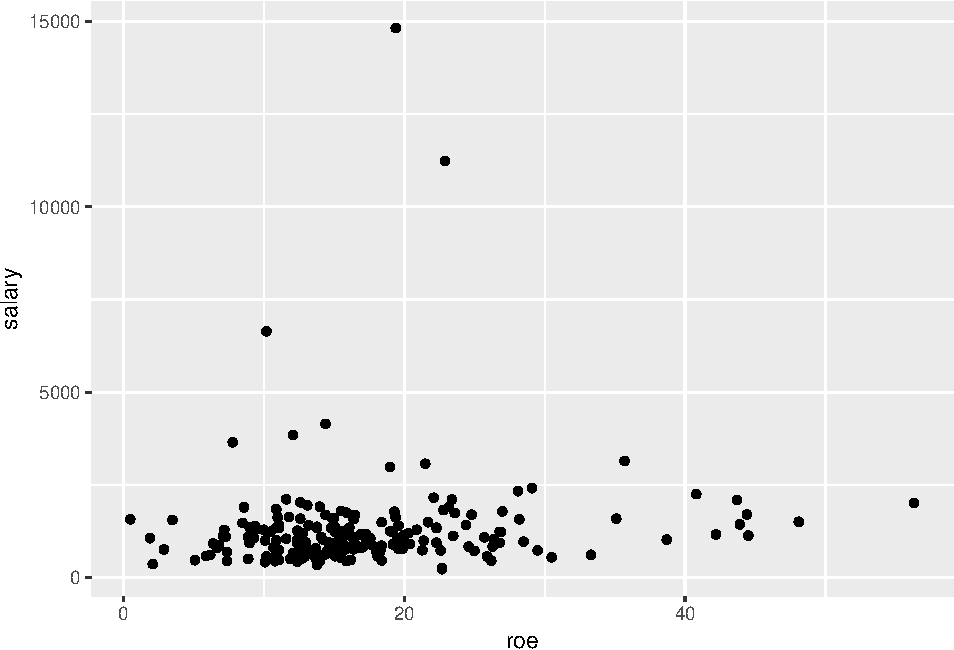
\includegraphics{MEM5220_R_files/figure-latex/ceosal1-1.pdf}
\caption{\label{fig:ceosal1}Relationship between ROE and Salary}
\end{figure}

Consider a simple regression model

\(salary = \beta_0 + \beta_1roe + u\)

We are concerned with the population parameter \(\beta_{0}\) and
\(\beta_{1}\). The general form of the model.

\begin{equation}
\hat{\beta}_{0} = \bar{y} - \hat{\beta}_{1}\bar{x}
\label{eq:populationparameterBeta0}
\end{equation}

The ordinary least squares (OLS) estimators are

\begin{equation}
\hat{\beta}_{0} = \bar{y} - \hat{\beta}_{1}\bar{x}
\label{eq:OLSestimator}
\end{equation}

Ingredients for the OLS formulas

\begin{Shaded}
\begin{Highlighting}[]
\KeywordTok{attach}\NormalTok{(ceosal1)}
\end{Highlighting}
\end{Shaded}

\begin{verbatim}
## The following objects are masked from ceosal1 (pos = 6):
## 
##     consprod, finance, indus, lsalary, lsales, pcroe, pcsalary,
##     roe, ros, salary, sales, utility
\end{verbatim}

\begin{Shaded}
\begin{Highlighting}[]
\KeywordTok{cov}\NormalTok{(roe, salary)}
\end{Highlighting}
\end{Shaded}

\begin{verbatim}
## [1] 1342.538
\end{verbatim}

\begin{Shaded}
\begin{Highlighting}[]
\KeywordTok{var}\NormalTok{(roe)}
\end{Highlighting}
\end{Shaded}

\begin{verbatim}
## [1] 72.56499
\end{verbatim}

\begin{Shaded}
\begin{Highlighting}[]
\KeywordTok{mean}\NormalTok{(salary)}
\end{Highlighting}
\end{Shaded}

\begin{verbatim}
## [1] 1281.12
\end{verbatim}

Manual calculation of the OLS coefficients

\begin{Shaded}
\begin{Highlighting}[]
\NormalTok{b1hat <-}\StringTok{ }\KeywordTok{cov}\NormalTok{(roe,salary)}\OperatorTok{/}\KeywordTok{var}\NormalTok{(roe)}
\end{Highlighting}
\end{Shaded}

\begin{Shaded}
\begin{Highlighting}[]
\NormalTok{b0hat <-}\StringTok{ }\KeywordTok{mean}\NormalTok{(salary) }\OperatorTok{-}\StringTok{ }\NormalTok{b1hat }\OperatorTok{*}\StringTok{ }\KeywordTok{mean}\NormalTok{(roe)}
\end{Highlighting}
\end{Shaded}

Or use the \texttt{lm()} function

\begin{Shaded}
\begin{Highlighting}[]
\KeywordTok{lm}\NormalTok{(salary }\OperatorTok{~}\StringTok{ }\NormalTok{roe, }\DataTypeTok{data=}\NormalTok{ceosal1)}
\end{Highlighting}
\end{Shaded}

\begin{verbatim}
## 
## Call:
## lm(formula = salary ~ roe, data = ceosal1)
## 
## Coefficients:
## (Intercept)          roe  
##       963.2         18.5
\end{verbatim}

\begin{Shaded}
\begin{Highlighting}[]
\NormalTok{lm1_ceosal1 <-}\StringTok{ }\KeywordTok{lm}\NormalTok{(salary }\OperatorTok{~}\StringTok{ }\NormalTok{roe, }\DataTypeTok{data=}\NormalTok{ceosal1) }
\end{Highlighting}
\end{Shaded}

\begin{Shaded}
\begin{Highlighting}[]
\KeywordTok{unique}\NormalTok{(ceosal1}\OperatorTok{$}\NormalTok{roe)}
\end{Highlighting}
\end{Shaded}

\begin{verbatim}
##   [1] 14.1 10.9 23.5  5.9 13.8 20.0 16.4 16.3 10.5 26.3 25.9 26.8 14.8 22.3
##  [15] 56.3 12.6 20.4  1.9 19.9 15.4 38.7 24.4 15.6 14.4 19.0 16.1 12.1 16.2
##  [29] 18.4 14.2 14.9 12.4 17.1 16.9 18.1 19.3 18.3 13.7 12.7 15.1 16.5 10.2
##  [43] 19.6 12.8 15.9 17.3  8.5 19.5 19.2 28.1 25.0 15.0 20.3 22.7 13.2 10.3
##  [57] 17.7 10.0  6.8 13.1 15.8 15.3  0.5 13.0 11.1  8.9 17.5  9.3  9.5 15.5
##  [71]  8.6 24.6  7.2 11.6 26.4 21.4  9.0  9.4  3.5 22.1 33.3 22.8 20.9  6.7
##  [85]  7.1 11.8 14.0 10.1  6.4 17.6 23.6 35.7 23.2 44.4  2.1 23.4 25.7 27.0
##  [99] 43.7 24.8 26.2 44.5 35.1 11.0 19.4 28.5 43.9 15.7 28.2 42.2 21.5 29.5
## [113] 22.6 22.9  7.8 48.1 18.0 21.7 21.3 26.9 30.5 29.1 40.8 10.8  5.1 12.3
## [127]  7.4  6.2 10.6  2.9 13.5 10.7 11.9 12.9  7.3 14.6 14.5 14.7
\end{verbatim}

Plot the linear regression fit the \emph{base} r way.

\begin{Shaded}
\begin{Highlighting}[]
\KeywordTok{plot}\NormalTok{(salary}\OperatorTok{~}\StringTok{ }\NormalTok{roe, }\DataTypeTok{data =}\NormalTok{ ceosal1,}
     \DataTypeTok{xlab =} \StringTok{"Return on equity"}\NormalTok{,}
     \DataTypeTok{ylab =} \StringTok{"Salary"}\NormalTok{,}
     \DataTypeTok{main =} \StringTok{"Salary vs return on equity"}\NormalTok{,}
     \DataTypeTok{pch  =} \DecValTok{20}\NormalTok{,}
     \DataTypeTok{cex  =} \DecValTok{2}\NormalTok{,}
     \DataTypeTok{col  =} \StringTok{"grey"}\NormalTok{)}
\KeywordTok{abline}\NormalTok{(lm1_ceosal1, }\DataTypeTok{lwd =} \DecValTok{3}\NormalTok{, }\DataTypeTok{col =} \StringTok{"darkorange"}\NormalTok{)}
\end{Highlighting}
\end{Shaded}

\begin{figure}

{\centering 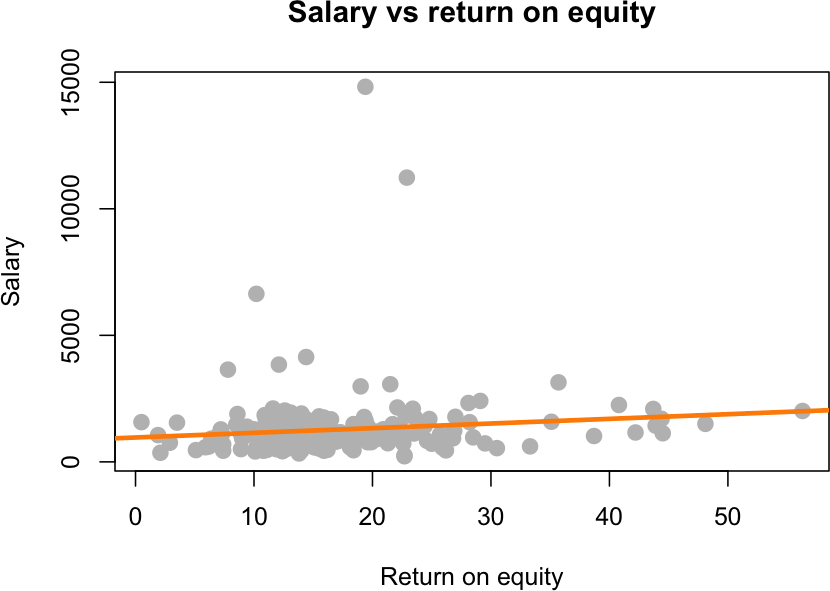
\includegraphics[width=0.8\linewidth]{MEM5220_R_files/figure-latex/fig1-1} 

}

\caption{OLS regression base Rstyle}\label{fig:fig1}
\end{figure}

Or use ggplot

\begin{Shaded}
\begin{Highlighting}[]
\KeywordTok{ggplot}\NormalTok{(ceosal1, }\KeywordTok{aes}\NormalTok{(}\DataTypeTok{x =}\NormalTok{ roe, }\DataTypeTok{y =}\NormalTok{ salary)) }\OperatorTok{+}\StringTok{ }
\StringTok{  }\KeywordTok{geom_point}\NormalTok{() }\OperatorTok{+}
\StringTok{  }\KeywordTok{stat_smooth}\NormalTok{(}\DataTypeTok{method =} \StringTok{"lm"}\NormalTok{, }\DataTypeTok{col =} \StringTok{"red"}\NormalTok{)}
\end{Highlighting}
\end{Shaded}

\begin{figure}

{\centering 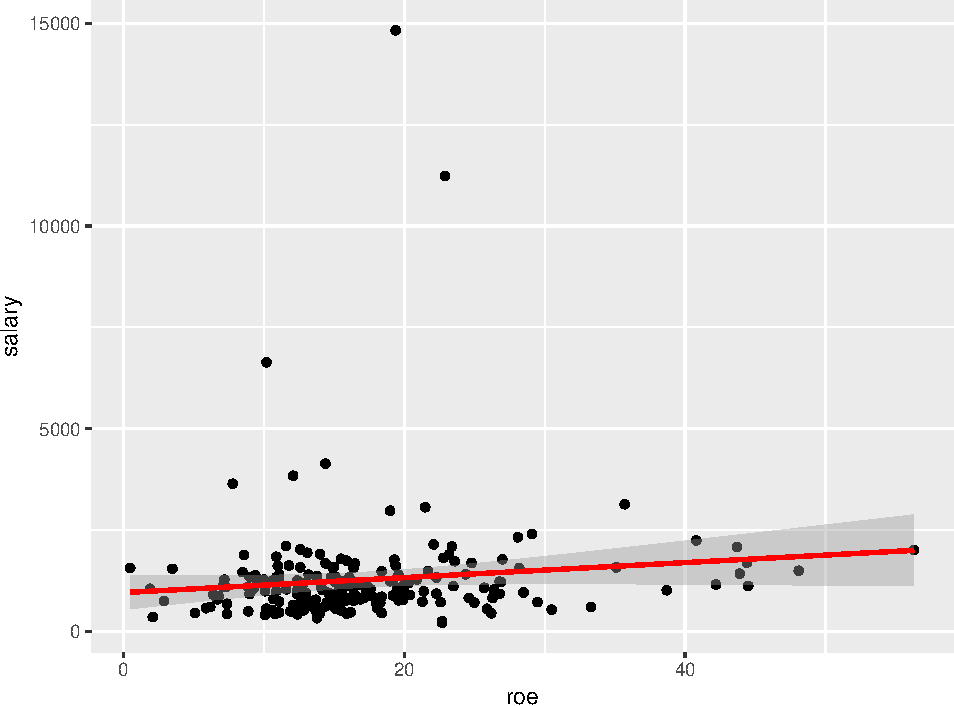
\includegraphics[width=0.8\linewidth]{MEM5220_R_files/figure-latex/fig2-1} 

}

\caption{OLS regression ggplot2 style}\label{fig:fig2}
\end{figure}

Determine the names of the elements of the list using the
\texttt{names()} command.

\begin{Shaded}
\begin{Highlighting}[]
\KeywordTok{names}\NormalTok{(lm1_ceosal1)}
\end{Highlighting}
\end{Shaded}

\begin{verbatim}
##  [1] "coefficients"  "residuals"     "effects"       "rank"         
##  [5] "fitted.values" "assign"        "qr"            "df.residual"  
##  [9] "xlevels"       "call"          "terms"         "model"
\end{verbatim}

Extract one element, for example the residuals from the list object

\begin{Shaded}
\begin{Highlighting}[]
\KeywordTok{head}\NormalTok{(lm1_ceosal1}\OperatorTok{$}\NormalTok{residuals) }\CommentTok{# head() just prints out the first 6 residual values}
\end{Highlighting}
\end{Shaded}

\begin{verbatim}
##         1         2         3         4         5         6 
## -129.0581 -163.8543 -275.9692 -494.3483  149.4923 -188.2151
\end{verbatim}

Another way to access stored information in \emph{lm1\_ceosal1} are the
\texttt{coef()}, \texttt{resid()}, and \texttt{fitted()} functions.
These return the coefficients, residuals, and fitted values,
respectively.

\begin{Shaded}
\begin{Highlighting}[]
\KeywordTok{coef}\NormalTok{(lm1_ceosal1)}
\end{Highlighting}
\end{Shaded}

\begin{verbatim}
## (Intercept)         roe 
##   963.19134    18.50119
\end{verbatim}

The function \texttt{summary()} is useful in many situations. We see
that when it is called on our model, it returns a good deal of
information.

\begin{Shaded}
\begin{Highlighting}[]
\KeywordTok{summary}\NormalTok{(lm1_ceosal1)}
\end{Highlighting}
\end{Shaded}

\begin{verbatim}
## 
## Call:
## lm(formula = salary ~ roe, data = ceosal1)
## 
## Residuals:
##     Min      1Q  Median      3Q     Max 
## -1160.2  -526.0  -254.0   138.8 13499.9 
## 
## Coefficients:
##             Estimate Std. Error t value Pr(>|t|)    
## (Intercept)   963.19     213.24   4.517 1.05e-05 ***
## roe            18.50      11.12   1.663   0.0978 .  
## ---
## Signif. codes:  0 '***' 0.001 '**' 0.01 '*' 0.05 '.' 0.1 ' ' 1
## 
## Residual standard error: 1367 on 207 degrees of freedom
## Multiple R-squared:  0.01319,    Adjusted R-squared:  0.008421 
## F-statistic: 2.767 on 1 and 207 DF,  p-value: 0.09777
\end{verbatim}

The \texttt{summary()} command also returns a list, and we can again use
\texttt{names()} to learn what about the elements of this list.

\begin{Shaded}
\begin{Highlighting}[]
\KeywordTok{names}\NormalTok{(}\KeywordTok{summary}\NormalTok{(lm1_ceosal1))}
\end{Highlighting}
\end{Shaded}

\begin{verbatim}
##  [1] "call"          "terms"         "residuals"     "coefficients" 
##  [5] "aliased"       "sigma"         "df"            "r.squared"    
##  [9] "adj.r.squared" "fstatistic"    "cov.unscaled"
\end{verbatim}

So, for example, if we wanted to directly access the value of \(R^2\),
instead of copy and pasting it out of the printed statement from
\texttt{summary()}, we could do so.

\begin{Shaded}
\begin{Highlighting}[]
\KeywordTok{summary}\NormalTok{(lm1_ceosal1)}\OperatorTok{$}\NormalTok{r.squared}
\end{Highlighting}
\end{Shaded}

\begin{verbatim}
## [1] 0.01318862
\end{verbatim}

\begin{center}\rule{0.5\linewidth}{\linethickness}\end{center}

\textbf{Your turn}

Recall that the residual sum of squares (SSR) is

\begin{equation}
R^2 = \frac{Var(\hat{y})}{Var(y)} = 1 - \frac{Var(\hat{u})}{Var(y)} 
\end{equation}

Calculate \(R^2\) manually:

\begin{Shaded}
\begin{Highlighting}[]
\KeywordTok{var}\NormalTok{(}\KeywordTok{fitted}\NormalTok{(lm1_ceosal1))}\OperatorTok{/}\KeywordTok{var}\NormalTok{(ceosal1}\OperatorTok{$}\NormalTok{salary)}
\end{Highlighting}
\end{Shaded}

\begin{verbatim}
## [1] 0.01318862
\end{verbatim}

\begin{Shaded}
\begin{Highlighting}[]
\DecValTok{1} \OperatorTok{-}\StringTok{ }\KeywordTok{var}\NormalTok{(}\KeywordTok{residuals}\NormalTok{(lm1_ceosal1))}\OperatorTok{/}\KeywordTok{var}\NormalTok{(ceosal1}\OperatorTok{$}\NormalTok{salary)}
\end{Highlighting}
\end{Shaded}

\begin{verbatim}
## [1] 0.01318862
\end{verbatim}

\begin{center}\rule{0.5\linewidth}{\linethickness}\end{center}

Another useful function is the \texttt{predict()} function.

\begin{Shaded}
\begin{Highlighting}[]
\KeywordTok{set.seed}\NormalTok{(}\DecValTok{123}\NormalTok{)}
\NormalTok{roe_sample <-}\KeywordTok{sample}\NormalTok{(ceosal1}\OperatorTok{$}\NormalTok{roe, }\DecValTok{1}\NormalTok{)}
\end{Highlighting}
\end{Shaded}

Let's make a prediction for salary when the return on equity is
20.2999992.

\begin{Shaded}
\begin{Highlighting}[]
\NormalTok{b0hat_sample <-}\StringTok{ }\KeywordTok{mean}\NormalTok{(salary) }\OperatorTok{-}\StringTok{ }\NormalTok{b1hat }\OperatorTok{*}\StringTok{ }\NormalTok{roe_sample }
\end{Highlighting}
\end{Shaded}

We are not restricted to observed values of the explanatory variable.
Instead we can supply also our own predictor values

\begin{Shaded}
\begin{Highlighting}[]
\KeywordTok{predict}\NormalTok{(lm1_ceosal1, }\DataTypeTok{newdata =} \KeywordTok{data.frame}\NormalTok{(}\DataTypeTok{roe =} \DecValTok{30}\NormalTok{))}
\end{Highlighting}
\end{Shaded}

\begin{verbatim}
##        1 
## 1518.227
\end{verbatim}

The above code reads ``predict the salary when the return on equity is
30 using the \emph{lm1\_ceosal1} model.''

\hypertarget{regression-through-the-origin-and-regression-on-a-constant}{%
\subsection{Regression through the Origin and Regression on a
Constant}\label{regression-through-the-origin-and-regression-on-a-constant}}

Regression without intercept (through origin)

\begin{Shaded}
\begin{Highlighting}[]
\NormalTok{lm2 <-}\StringTok{ }\KeywordTok{lm}\NormalTok{(salary }\OperatorTok{~}\StringTok{  }\DecValTok{0} \OperatorTok{+}\StringTok{ }\NormalTok{roe, }\DataTypeTok{data =}\NormalTok{ ceosal1)}
\end{Highlighting}
\end{Shaded}

Regression without slope

\begin{Shaded}
\begin{Highlighting}[]
\NormalTok{lm3 <-}\StringTok{ }\KeywordTok{lm}\NormalTok{(salary }\OperatorTok{~}\StringTok{ }\DecValTok{1}\NormalTok{, }\DataTypeTok{data =}\NormalTok{ ceosal1)}
\end{Highlighting}
\end{Shaded}

\begin{Shaded}
\begin{Highlighting}[]
\KeywordTok{plot}\NormalTok{(salary}\OperatorTok{~}\StringTok{ }\NormalTok{roe, }\DataTypeTok{data =}\NormalTok{ ceosal1,}
     \DataTypeTok{xlab =} \StringTok{"Return on equity"}\NormalTok{,}
     \DataTypeTok{ylab =} \StringTok{"Salary"}\NormalTok{,}
     \DataTypeTok{main =} \StringTok{"Salary vs return on equity"}\NormalTok{,}
     \DataTypeTok{pch  =} \DecValTok{20}\NormalTok{,}
     \DataTypeTok{cex  =} \DecValTok{2}\NormalTok{,}
     \DataTypeTok{col  =} \StringTok{"grey"}\NormalTok{)}
\KeywordTok{abline}\NormalTok{(lm1_ceosal1, }\DataTypeTok{lwd =} \DecValTok{3}\NormalTok{, }\DataTypeTok{lty =} \DecValTok{1}\NormalTok{, }\DataTypeTok{col =} \StringTok{"darkorange"}\NormalTok{)}
\KeywordTok{abline}\NormalTok{(lm2,}\DataTypeTok{lwd =} \DecValTok{3}\NormalTok{,  }\DataTypeTok{lty =} \DecValTok{2}\NormalTok{,   }\DataTypeTok{col =} \StringTok{"darkblue"}\NormalTok{)}
\KeywordTok{abline}\NormalTok{(lm3, }\DataTypeTok{lwd =} \DecValTok{3}\NormalTok{,  }\DataTypeTok{lty =} \DecValTok{3}\NormalTok{,   }\DataTypeTok{col =} \StringTok{"black"}\NormalTok{)}
\KeywordTok{legend}\NormalTok{(}\StringTok{"topleft"}\NormalTok{, }
       \KeywordTok{c}\NormalTok{(}\StringTok{"full"}\NormalTok{, }
         \StringTok{"through origin"}\NormalTok{, }
         \StringTok{"constant only"}\NormalTok{), }
       \DataTypeTok{lwd =}\DecValTok{2}\NormalTok{, }
       \DataTypeTok{lty =} \DecValTok{1}\OperatorTok{:}\DecValTok{3}\NormalTok{)}
\end{Highlighting}
\end{Shaded}

\begin{figure}

{\centering 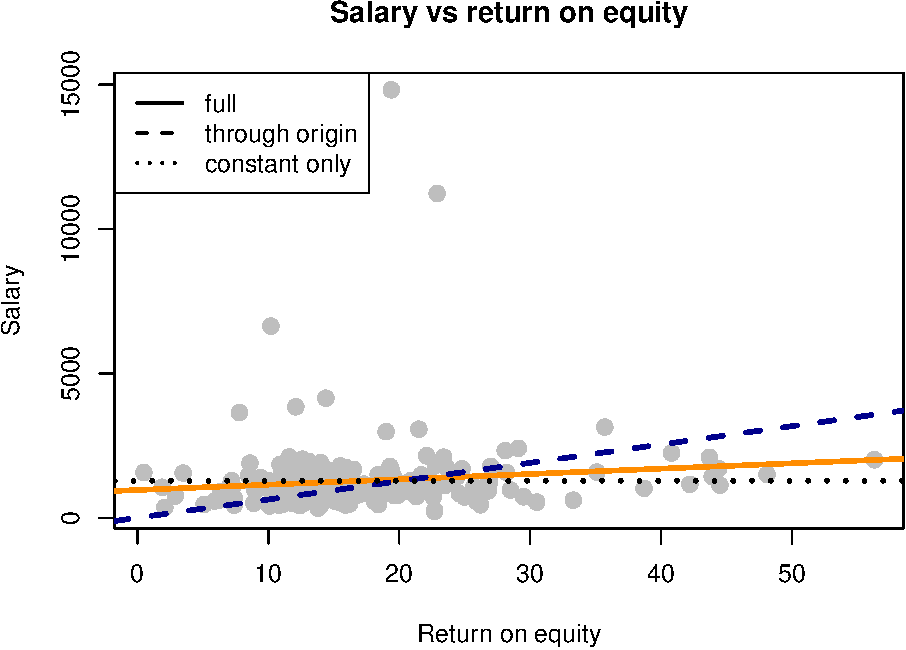
\includegraphics[width=0.8\linewidth]{MEM5220_R_files/figure-latex/fig3-1} 

}

\caption{Regression through the Origin and on a Constant}\label{fig:fig3}
\end{figure}

\hypertarget{simulating-slr}{%
\subsection{Simulating SLR}\label{simulating-slr}}

\hypertarget{expected-values-variance-and-standard-errors}{%
\paragraph{Expected Values, Variance, and Standard
Errors}\label{expected-values-variance-and-standard-errors}}

The \textbf{Gauss--Markov theorem} tells us that when estimating the
parameters of the simple linear regression model \(\beta_{0}\) and
\(\beta_{1}\), the \(\hat{\beta}_{0}\) and \(\hat{\beta}_{1}\) which we
derived are the best linear unbiased estimates, or BLUE for short. (The
actual conditions for the Gauss--Markov theorem are more relaxed than
the SLR model.)

In short those assumptions are:

\begin{itemize}
\tightlist
\item
  SLR.1 Linear population regression function
  \(y = \beta_0 + \beta_{1} \times x + u\)
\item
  SLR.2 Random sampling of x and y from the population\\
\item
  SLR.3 Variation in the sample values: \(x_{1}, \dots , x_{n}\)
\item
  SLR.4 Zero conditional mean: \(\mathbf{E}(u|x) = 0\)
\item
  SLR.5 Homeskedasticity: \(Var(u|x) = \sigma^2\)
\end{itemize}

Recall that under \textbf{SLR.1 - SLR.4} the OLS parameter estimators
are unbiased. Under \textbf{SLR.1 - SLR.4} the OLS parameter estimators
have a specific sampling variance.

Simulating a model is an important concept. In practice you will almost
never have a true model, and you will use data to attempt to recover
information about the unknown true model. With simulation, we decide the
true model and simulate data from it. Then, we apply a method to the
data, in this case least squares. Now, since we know the true model, we
can assess how well it did.

Simulation also helps to grasp the concepts of estimators, estimates,
unbiasedness, the sampling variance of the estimators, and the
consequences of violated assumptions.

Sample size

\begin{Shaded}
\begin{Highlighting}[]
\NormalTok{n <-}\StringTok{ }\DecValTok{200}
\end{Highlighting}
\end{Shaded}

True parameters

\begin{Shaded}
\begin{Highlighting}[]
\NormalTok{b0<-}\StringTok{ }\DecValTok{1}
\NormalTok{b1 <-}\StringTok{ }\FloatTok{0.5}
\NormalTok{sigma <-}\StringTok{ }\DecValTok{2} \CommentTok{# standard deviation of the error term u }
\NormalTok{x1 <-}\StringTok{ }\DecValTok{5}
\end{Highlighting}
\end{Shaded}

Determine the distribution of the independent variable

\begin{Shaded}
\begin{Highlighting}[]
\NormalTok{yhat1 <-}\StringTok{ }\NormalTok{b0 }\OperatorTok{+}\StringTok{ }\NormalTok{b1 }\OperatorTok{*}\StringTok{ }\NormalTok{x1 }\CommentTok{#  Note that we do not include the error term }
\end{Highlighting}
\end{Shaded}

Plot a Gaussian distribution of the dependent variable based on the
parameters

\begin{Shaded}
\begin{Highlighting}[]
\KeywordTok{curve}\NormalTok{(}\KeywordTok{dnorm}\NormalTok{(x, }\DataTypeTok{mean =}\NormalTok{ yhat1, }\DataTypeTok{sd =}\NormalTok{ sigma), }\DecValTok{-5}\NormalTok{, }\DecValTok{15}\NormalTok{, }\DataTypeTok{col =} \StringTok{"blue"}\NormalTok{)}
\KeywordTok{abline}\NormalTok{(}\DataTypeTok{v =}\NormalTok{ yhat1, }\DataTypeTok{col =} \StringTok{"blue"}\NormalTok{, }\DataTypeTok{lty =} \DecValTok{2}\NormalTok{)}
\KeywordTok{legend}\NormalTok{(}\StringTok{"topright"}\NormalTok{, }\DataTypeTok{legend =} \KeywordTok{c}\NormalTok{(}\StringTok{"f(y|x = 5)"}\NormalTok{), }\DataTypeTok{lty =} \DecValTok{1}\NormalTok{, }\DataTypeTok{col =} \KeywordTok{c}\NormalTok{(}\StringTok{"blue"}\NormalTok{))}
\end{Highlighting}
\end{Shaded}

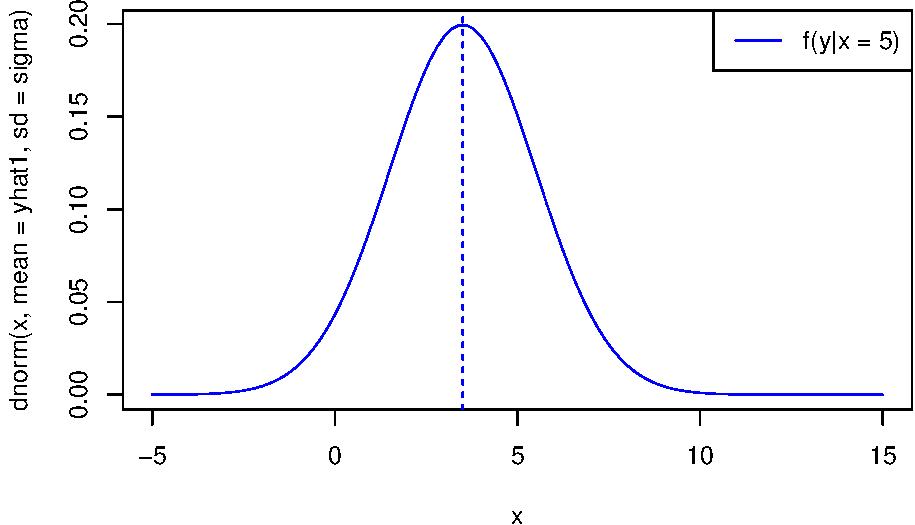
\includegraphics{MEM5220_R_files/figure-latex/unnamed-chunk-33-1.pdf}

This represent the theoretical (true) probability distribution of \(y\),
given \(x\)

We can calculate the variance of \(b_{1}\) and plot the corresponding
density function.

\begin{equation}
var(b_2) = \frac{\sigma^2}{\sum{}{}(x_1 - \bar{x})}
\label{eq:variancebeta}
\end{equation}

Assume that \(x_{2}\) represents a second possible predictor of \(y\)

\begin{Shaded}
\begin{Highlighting}[]
\NormalTok{x2 <-}\StringTok{ }\DecValTok{18}

\NormalTok{x <-}\StringTok{ }\KeywordTok{c}\NormalTok{(}\KeywordTok{rep}\NormalTok{(x1, n}\OperatorTok{/}\DecValTok{2}\NormalTok{), }\KeywordTok{rep}\NormalTok{(x2, n}\OperatorTok{/}\DecValTok{2}\NormalTok{))}
\NormalTok{xbar <-}\StringTok{ }\KeywordTok{mean}\NormalTok{(x)}

\NormalTok{sumxbar <-}\StringTok{ }\KeywordTok{sum}\NormalTok{((x}\OperatorTok{-}\NormalTok{xbar)}\OperatorTok{^}\DecValTok{2}\NormalTok{)}
\NormalTok{varb <-}\StringTok{ }\NormalTok{(sigma}\OperatorTok{^}\DecValTok{2}\NormalTok{)}\OperatorTok{/}\NormalTok{sumxbar}
\NormalTok{sdb <-}\KeywordTok{sqrt}\NormalTok{(varb)}
\NormalTok{leftlim <-}\StringTok{ }\NormalTok{b1}\DecValTok{-3}\OperatorTok{*}\NormalTok{sdb}
\NormalTok{rightlim <-}\StringTok{ }\NormalTok{b1}\OperatorTok{+}\DecValTok{3}\OperatorTok{*}\NormalTok{sdb}
\end{Highlighting}
\end{Shaded}

\begin{Shaded}
\begin{Highlighting}[]
\KeywordTok{curve}\NormalTok{(}\KeywordTok{dnorm}\NormalTok{(x, }\DataTypeTok{mean =}\NormalTok{ b1, }\DataTypeTok{sd =}\NormalTok{ sdb), leftlim, rightlim,)}
\KeywordTok{abline}\NormalTok{(}\DataTypeTok{v =}\NormalTok{ b1, }\DataTypeTok{col =} \StringTok{"blue"}\NormalTok{, }\DataTypeTok{lty =} \DecValTok{2}\NormalTok{)}
\end{Highlighting}
\end{Shaded}

\begin{figure}

{\centering 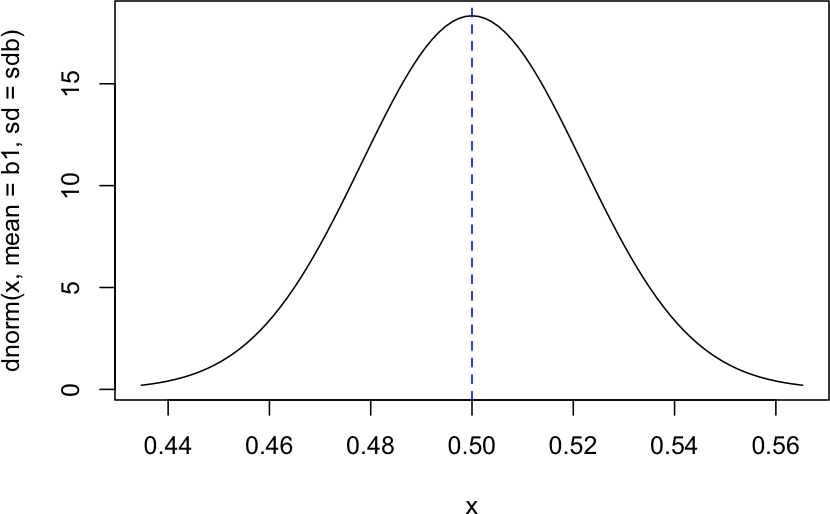
\includegraphics[width=0.8\linewidth]{MEM5220_R_files/figure-latex/fig4-1} 

}

\caption{The theoretical (true) probability density function of b1}\label{fig:fig4}
\end{figure}

Draw sample of size \(n\)

\begin{Shaded}
\begin{Highlighting}[]
\NormalTok{x <-}\StringTok{ }\KeywordTok{rnorm}\NormalTok{(n, }\DecValTok{4}\NormalTok{, sigma)}
\CommentTok{# Another way is to assume that the values for x are fixed and know}
\CommentTok{# x= seq(from = 0, to = 10, length.out = n)}
\end{Highlighting}
\end{Shaded}

\begin{Shaded}
\begin{Highlighting}[]
\NormalTok{u <-}\StringTok{ }\KeywordTok{rnorm}\NormalTok{(n, }\DecValTok{0}\NormalTok{, sigma)}
\end{Highlighting}
\end{Shaded}

\begin{Shaded}
\begin{Highlighting}[]
\NormalTok{y <-}\StringTok{ }\NormalTok{b0 }\OperatorTok{+}\StringTok{ }\NormalTok{b1 }\OperatorTok{*}\StringTok{ }\NormalTok{x }\OperatorTok{+}\StringTok{ }\NormalTok{u}
\end{Highlighting}
\end{Shaded}

Estimate parameter by OLS

\begin{Shaded}
\begin{Highlighting}[]
\NormalTok{olsreg <-}\StringTok{ }\KeywordTok{lm}\NormalTok{(y }\OperatorTok{~}\NormalTok{x )}
\end{Highlighting}
\end{Shaded}

\begin{Shaded}
\begin{Highlighting}[]
\NormalTok{simulation.df <-}\StringTok{ }\KeywordTok{data.frame}\NormalTok{(x,y)}
\NormalTok{population.df <-}\StringTok{ }\KeywordTok{data.frame}\NormalTok{(b0, b1)}
\end{Highlighting}
\end{Shaded}

\begin{Shaded}
\begin{Highlighting}[]
\KeywordTok{plot}\NormalTok{(simulation.df, }
     \DataTypeTok{xlab =} \StringTok{"x"}\NormalTok{,}
     \DataTypeTok{ylab =} \StringTok{"y"}\NormalTok{,}
     \CommentTok{# main = "Simulate least squares regression",}
     \DataTypeTok{pch  =} \DecValTok{20}\NormalTok{,}
     \DataTypeTok{cex  =} \DecValTok{2}\NormalTok{,}
     \DataTypeTok{col  =} \StringTok{"grey"}\NormalTok{)}
\KeywordTok{abline}\NormalTok{(olsreg, }\DataTypeTok{lwd =} \DecValTok{3}\NormalTok{, }\DataTypeTok{lty =} \DecValTok{1}\NormalTok{, }\DataTypeTok{col =} \StringTok{"darkorange"}\NormalTok{)}
\KeywordTok{abline}\NormalTok{(b0, b1,  }\DataTypeTok{lwd =} \DecValTok{3}\NormalTok{,  }\DataTypeTok{lty =} \DecValTok{2}\NormalTok{,   }\DataTypeTok{col =} \StringTok{"darkblue"}\NormalTok{)}
\KeywordTok{legend}\NormalTok{(}\StringTok{"topleft"}\NormalTok{, }
       \KeywordTok{c}\NormalTok{(}\StringTok{"OLS regression function"}\NormalTok{, }
         \StringTok{"Population regression function"}\NormalTok{), }
       \DataTypeTok{lwd =}\DecValTok{2}\NormalTok{, }
       \DataTypeTok{lty =} \DecValTok{1}\OperatorTok{:}\DecValTok{2}\NormalTok{)}
\end{Highlighting}
\end{Shaded}

\begin{figure}

{\centering 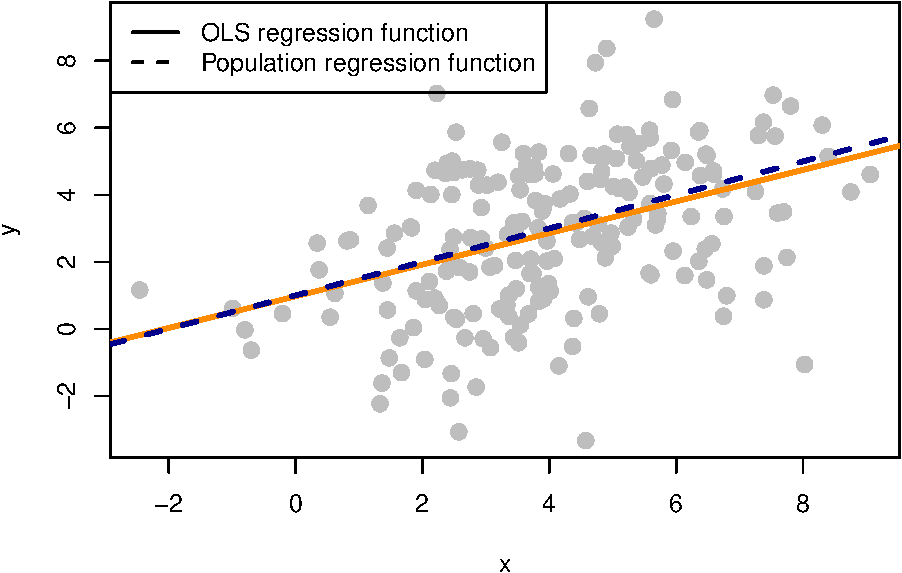
\includegraphics[width=0.8\linewidth]{MEM5220_R_files/figure-latex/fig5-1} 

}

\caption{Simulated Sample and OLS Regression Line}\label{fig:fig5}
\end{figure}

\begin{Shaded}
\begin{Highlighting}[]
\NormalTok{lable1 <-}\StringTok{ "OLS regression function"}
\KeywordTok{ggplot}\NormalTok{(simulation.df, }\KeywordTok{aes}\NormalTok{(}\DataTypeTok{x =}\NormalTok{ x,  }\DataTypeTok{y =}\NormalTok{ y)) }\OperatorTok{+}
\StringTok{  }\KeywordTok{geom_point}\NormalTok{() }\OperatorTok{+}
\StringTok{  }\KeywordTok{geom_abline}\NormalTok{(}\KeywordTok{aes}\NormalTok{(}\DataTypeTok{intercept=}\NormalTok{b0,}\DataTypeTok{slope=}\NormalTok{b1,}\DataTypeTok{colour=}\StringTok{"Population regression function"}\NormalTok{), }\DataTypeTok{linetype =}\StringTok{"dashed"}\NormalTok{, }\DataTypeTok{show.legend  =} \OtherTok{TRUE}\NormalTok{)}\OperatorTok{+}
\StringTok{  }\KeywordTok{stat_smooth}\NormalTok{(}\KeywordTok{aes}\NormalTok{(}\DataTypeTok{colour =}\StringTok{"OLS regression function"}\NormalTok{), }\DataTypeTok{method =} \StringTok{"lm"}\NormalTok{,}\DataTypeTok{se=}\OtherTok{FALSE}\NormalTok{, }\DataTypeTok{show.legend =}\OtherTok{TRUE}\NormalTok{)}\OperatorTok{+}
\StringTok{  }\KeywordTok{labs}\NormalTok{(}\DataTypeTok{colour =} \StringTok{"Regression functions"} 
       \CommentTok{# , title = "Simulate least squares regression"}
\NormalTok{       ) }\OperatorTok{+}
\StringTok{  }\KeywordTok{theme_bw}\NormalTok{()}
\end{Highlighting}
\end{Shaded}

\begin{figure}

{\centering 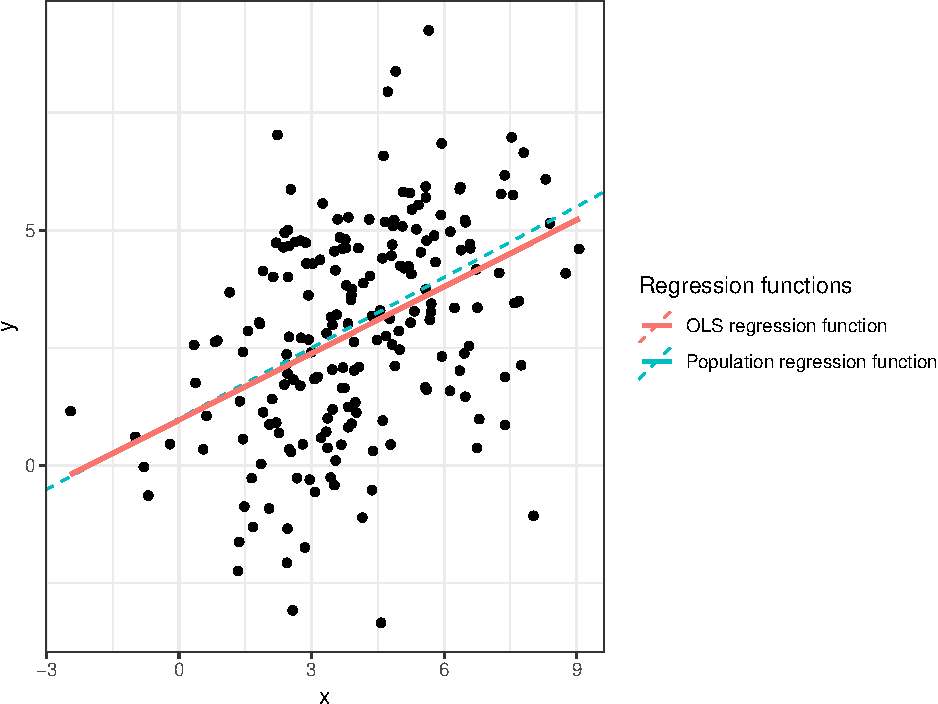
\includegraphics[width=0.8\linewidth]{MEM5220_R_files/figure-latex/fig6-1} 

}

\caption{Simulated Sample and OLS Regression Line (gpplot Style)}\label{fig:fig6}
\end{figure}

Since the expected values and variances of our estimators are defined
over separate random samples from the same population, it makes sense to
repeat our simulation exercise over many simulated samples.

\begin{Shaded}
\begin{Highlighting}[]
\CommentTok{# Set the random seed}
\KeywordTok{set.seed}\NormalTok{(}\DecValTok{1234567}\NormalTok{)}

\CommentTok{# set sample size and number of simulations}
\NormalTok{n<-}\DecValTok{1000}\NormalTok{; r<-}\DecValTok{10000}

\CommentTok{# set true parameters: betas and sd of u}
\NormalTok{b0<-}\FloatTok{1.0}\NormalTok{; b1<-}\FloatTok{0.5}\NormalTok{; sigma<-}\DecValTok{2}

\CommentTok{# initialize b0hat and b1hat to store results later:}
\NormalTok{b0hat <-}\StringTok{ }\KeywordTok{numeric}\NormalTok{(r)}
\NormalTok{b1hat <-}\StringTok{ }\KeywordTok{numeric}\NormalTok{(r)}

\CommentTok{# Draw a sample of x, fixed over replications:}
\NormalTok{x <-}\StringTok{ }\KeywordTok{rnorm}\NormalTok{(n,}\DecValTok{4}\NormalTok{,}\DecValTok{1}\NormalTok{)}

\CommentTok{# repeat r times:}
\ControlFlowTok{for}\NormalTok{(j }\ControlFlowTok{in} \DecValTok{1}\OperatorTok{:}\NormalTok{r) \{}
  \CommentTok{# Draw a sample of y:}
\NormalTok{  u <-}\StringTok{ }\KeywordTok{rnorm}\NormalTok{(n,}\DecValTok{0}\NormalTok{,sigma)}
\NormalTok{  y <-}\StringTok{ }\NormalTok{b0 }\OperatorTok{+}\StringTok{ }\NormalTok{b1}\OperatorTok{*}\NormalTok{x }\OperatorTok{+}\StringTok{ }\NormalTok{u}
  
  \CommentTok{# estimate parameters by OLS and store them in the vectors}
\NormalTok{  bhat <-}\StringTok{ }\KeywordTok{coefficients}\NormalTok{( }\KeywordTok{lm}\NormalTok{(y}\OperatorTok{~}\NormalTok{x) )}
\NormalTok{  b0hat[j] <-}\StringTok{ }\NormalTok{bhat[}\StringTok{"(Intercept)"}\NormalTok{]}
\NormalTok{  b1hat[j] <-}\StringTok{ }\NormalTok{bhat[}\StringTok{"x"}\NormalTok{]}
\NormalTok{\}}
\end{Highlighting}
\end{Shaded}

\begin{Shaded}
\begin{Highlighting}[]
\CommentTok{# MC estimate of the expected values:}
\KeywordTok{mean}\NormalTok{(b0hat)}
\end{Highlighting}
\end{Shaded}

\begin{verbatim}
## [1] 0.9985388
\end{verbatim}

\begin{Shaded}
\begin{Highlighting}[]
\KeywordTok{mean}\NormalTok{(b1hat)}
\end{Highlighting}
\end{Shaded}

\begin{verbatim}
## [1] 0.5000466
\end{verbatim}

\begin{Shaded}
\begin{Highlighting}[]
\CommentTok{# MC estimate of the variances:}
\KeywordTok{var}\NormalTok{(b0hat)}
\end{Highlighting}
\end{Shaded}

\begin{verbatim}
## [1] 0.0690833
\end{verbatim}

\begin{Shaded}
\begin{Highlighting}[]
\KeywordTok{var}\NormalTok{(b1hat)}
\end{Highlighting}
\end{Shaded}

\begin{verbatim}
## [1] 0.004069063
\end{verbatim}

\begin{Shaded}
\begin{Highlighting}[]
\CommentTok{# Initialize empty plot}
\KeywordTok{plot}\NormalTok{( }\OtherTok{NULL}\NormalTok{, }\DataTypeTok{xlim=}\KeywordTok{c}\NormalTok{(}\DecValTok{0}\NormalTok{,}\DecValTok{8}\NormalTok{), }\DataTypeTok{ylim=}\KeywordTok{c}\NormalTok{(}\DecValTok{0}\NormalTok{,}\DecValTok{6}\NormalTok{), }\DataTypeTok{xlab=}\StringTok{"x"}\NormalTok{, }\DataTypeTok{ylab=}\StringTok{"y"}\NormalTok{)}
\CommentTok{# add OLS regression lines}
\ControlFlowTok{for}\NormalTok{ (j }\ControlFlowTok{in} \DecValTok{1}\OperatorTok{:}\DecValTok{10}\NormalTok{) }\KeywordTok{abline}\NormalTok{(b0hat[j],b1hat[j],}\DataTypeTok{col=}\StringTok{"gray"}\NormalTok{)}
\CommentTok{# add population regression line}
\KeywordTok{abline}\NormalTok{(b0,b1,}\DataTypeTok{lwd=}\DecValTok{2}\NormalTok{)}
\CommentTok{# add legend}
\KeywordTok{legend}\NormalTok{(}\StringTok{"topleft"}\NormalTok{,}\KeywordTok{c}\NormalTok{(}\StringTok{"Population"}\NormalTok{,}\StringTok{"OLS regressions"}\NormalTok{),}
       \DataTypeTok{lwd=}\KeywordTok{c}\NormalTok{(}\DecValTok{2}\NormalTok{,}\DecValTok{1}\NormalTok{),}\DataTypeTok{col=}\KeywordTok{c}\NormalTok{(}\StringTok{"black"}\NormalTok{,}\StringTok{"gray"}\NormalTok{))}
\end{Highlighting}
\end{Shaded}

\begin{figure}

{\centering 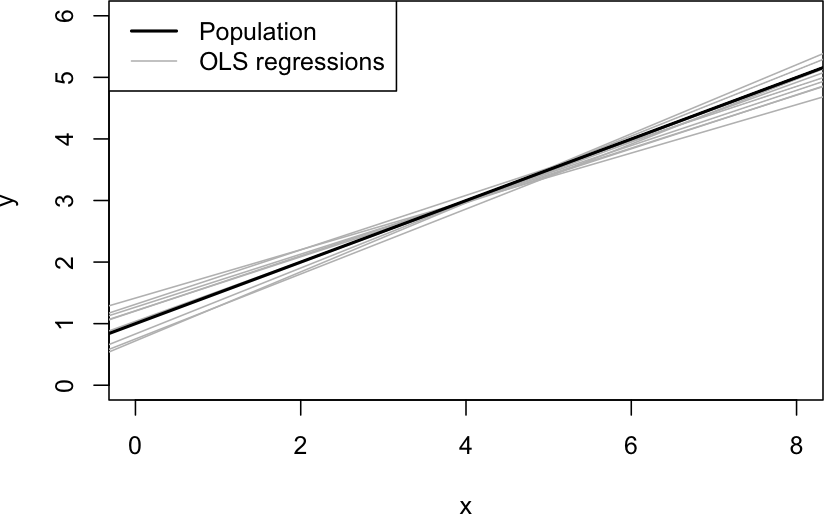
\includegraphics[width=0.8\linewidth]{MEM5220_R_files/figure-latex/fig7-1} 

}

\caption{Population and Simulated OLS Regression Lines}\label{fig:fig7}
\end{figure}

Even though the loop solution is transparent, let us take a look at a
different, more \emph{modern} approach.

\begin{Shaded}
\begin{Highlighting}[]
\CommentTok{# define a function the returns the alpha -- its point estimate, standard error, etc. -- from the OLS}
\NormalTok{x <-}\StringTok{ }\KeywordTok{rnorm}\NormalTok{(n,}\DecValTok{4}\NormalTok{,}\DecValTok{1}\NormalTok{) }\CommentTok{# }\AlertTok{NOTE}\CommentTok{ 1: Although a normal distribution is usually defined by its mean and variance, 'rnorm()' requires the standard deviation as input for the second moment.}
\CommentTok{# }\AlertTok{NOTE}\CommentTok{ 2: We use the same values for x in all samples since we draw them outside of the loop. }

\NormalTok{iteration <-}\StringTok{ }\ControlFlowTok{function}\NormalTok{() \{}
\NormalTok{  u <-}\StringTok{ }\KeywordTok{rnorm}\NormalTok{(n,}\DecValTok{0}\NormalTok{,sigma)}
\NormalTok{  y <-}\StringTok{ }\NormalTok{b0 }\OperatorTok{+}\StringTok{ }\NormalTok{b1}\OperatorTok{*}\NormalTok{x }\OperatorTok{+}\StringTok{ }\NormalTok{u}
  
  \KeywordTok{lm}\NormalTok{(y}\OperatorTok{~}\NormalTok{x) }\OperatorTok\StringTok{ }
\StringTok{    }\NormalTok{broom}\OperatorTok{::}\KeywordTok{tidy}\NormalTok{() }\CommentTok{# %>% }
  \CommentTok{# filter(term == 'x') # One could only extract the slope}
\NormalTok{\}}

\CommentTok{# 1000 iterations of the above simulation}
\NormalTok{MC_coef<-}\StringTok{ }\KeywordTok{map_df}\NormalTok{(}\DecValTok{1}\OperatorTok{:}\DecValTok{1000}\NormalTok{, }\OperatorTok{~}\KeywordTok{iteration}\NormalTok{()) }
\KeywordTok{str}\NormalTok{(MC_coef)}
\end{Highlighting}
\end{Shaded}

\begin{verbatim}
## Classes 'tbl_df', 'tbl' and 'data.frame':    2000 obs. of  5 variables:
##  $ term     : chr  "(Intercept)" "x" "(Intercept)" "x" ...
##  $ estimate : num  1.577 0.372 1.44 0.387 1.355 ...
##  $ std.error: num  0.2672 0.0639 0.2623 0.0628 0.2626 ...
##  $ statistic: num  5.9 5.82 5.49 6.17 5.16 ...
##  $ p.value  : num  4.94e-09 7.91e-09 5.13e-08 9.92e-10 2.99e-07 ...
\end{verbatim}

Instead of plotting simulated and true parameter regression lines we can
take a look at the kernel density of the simulated parameter estimates

Figure \ref{fig:fig8} shows the simulated distribution of \(\beta_{0}\)
and \(\beta_{1}\) the theoretical one.

\begin{Shaded}
\begin{Highlighting}[]
\CommentTok{# plot the results}
\KeywordTok{str}\NormalTok{(MC_coef)}
\end{Highlighting}
\end{Shaded}

\begin{verbatim}
## Classes 'tbl_df', 'tbl' and 'data.frame':    2000 obs. of  5 variables:
##  $ term     : chr  "(Intercept)" "x" "(Intercept)" "x" ...
##  $ estimate : num  1.577 0.372 1.44 0.387 1.355 ...
##  $ std.error: num  0.2672 0.0639 0.2623 0.0628 0.2626 ...
##  $ statistic: num  5.9 5.82 5.49 6.17 5.16 ...
##  $ p.value  : num  4.94e-09 7.91e-09 5.13e-08 9.92e-10 2.99e-07 ...
\end{verbatim}

\begin{Shaded}
\begin{Highlighting}[]
\NormalTok{MC_coef<-}\StringTok{ }\NormalTok{MC_coef }\OperatorTok
\StringTok{  }\KeywordTok{mutate}\NormalTok{(}\DataTypeTok{OLScoeff =}  \KeywordTok{ifelse}\NormalTok{(term }\OperatorTok{==}\StringTok{ "x"}\NormalTok{, }\StringTok{"b1hat"}\NormalTok{, }\StringTok{"b0hat"}\NormalTok{)) }\OperatorTok\StringTok{  }\CommentTok{# rename the x to b1hat and (Intercept) to b0hat and create a new column }
\StringTok{  }\KeywordTok{mutate}\NormalTok{(}\DataTypeTok{Simulated =} \KeywordTok{ifelse}\NormalTok{(term }\OperatorTok{==}\StringTok{ "x"}\NormalTok{, }\StringTok{"b1"}\NormalTok{, }\StringTok{"b0"}\NormalTok{)) }\CommentTok{#  %>% }
\end{Highlighting}
\end{Shaded}

\begin{Shaded}
\begin{Highlighting}[]
\KeywordTok{ggplot}\NormalTok{(}\DataTypeTok{data=}\NormalTok{ MC_coef, }\KeywordTok{aes}\NormalTok{(estimate)) }\OperatorTok{+}\StringTok{ }
\StringTok{  }\KeywordTok{geom_histogram}\NormalTok{() }\OperatorTok{+}\StringTok{ }
\StringTok{  }\KeywordTok{geom_vline}\NormalTok{(}\DataTypeTok{data =} \KeywordTok{filter}\NormalTok{(MC_coef, OLScoeff }\OperatorTok{==}\StringTok{ "b0hat"}\NormalTok{), }\KeywordTok{aes}\NormalTok{(}\DataTypeTok{xintercept=}\NormalTok{b0), }\DataTypeTok{colour=}\StringTok{"pink"}\NormalTok{) }\OperatorTok{+}
\StringTok{  }\KeywordTok{geom_vline}\NormalTok{(}\DataTypeTok{data =} \KeywordTok{filter}\NormalTok{(MC_coef, OLScoeff }\OperatorTok{==}\StringTok{ "b1hat"}\NormalTok{), }\KeywordTok{aes}\NormalTok{(}\DataTypeTok{xintercept=}\NormalTok{b1), }\DataTypeTok{colour=}\StringTok{"darkgreen"}\NormalTok{) }\OperatorTok{+}\StringTok{ }
\StringTok{  }\KeywordTok{geom_text}\NormalTok{(}\DataTypeTok{data=}\NormalTok{MC_coef[}\DecValTok{3}\NormalTok{,], }\DataTypeTok{mapping=}\KeywordTok{aes}\NormalTok{(}\DataTypeTok{x=}\NormalTok{estimate, }\DataTypeTok{y=}\DecValTok{8}\NormalTok{, }\DataTypeTok{label=}\KeywordTok{paste}\NormalTok{(}\StringTok{"True parameter: "}\NormalTok{, MC_coef[}\DecValTok{3}\NormalTok{,}\DecValTok{7}\NormalTok{])), }\DataTypeTok{colour =} \StringTok{"pink"}\NormalTok{) }\OperatorTok{+}
\StringTok{  }\KeywordTok{geom_text}\NormalTok{(}\DataTypeTok{data=}\NormalTok{MC_coef[}\DecValTok{4}\NormalTok{,], }\DataTypeTok{mapping=}\KeywordTok{aes}\NormalTok{(}\DataTypeTok{x=}\NormalTok{estimate, }\DataTypeTok{y=}\DecValTok{8}\NormalTok{, }\DataTypeTok{label=}\KeywordTok{paste}\NormalTok{(}\StringTok{"True parameter: "}\NormalTok{, MC_coef[}\DecValTok{4}\NormalTok{,}\DecValTok{7}\NormalTok{])), }\DataTypeTok{colour =} \StringTok{"darkgreen"}\NormalTok{) }\OperatorTok{+}
\StringTok{  }\KeywordTok{facet_wrap}\NormalTok{( }\OperatorTok{~}\StringTok{ }\NormalTok{OLScoeff, }\DataTypeTok{scales =} \StringTok{"free"}\NormalTok{)   }\OperatorTok{+}
\StringTok{  }\KeywordTok{labs}\NormalTok{(}
    \DataTypeTok{title =} \StringTok{"Histogram Monte Carlo Simulations and True population parameters"}\NormalTok{) }\OperatorTok{+}
\StringTok{  }\KeywordTok{theme_bw}\NormalTok{()}
\end{Highlighting}
\end{Shaded}

\begin{verbatim}
## `stat_bin()` using `bins = 30`. Pick better value with `binwidth`.
\end{verbatim}

\begin{figure}

{\centering 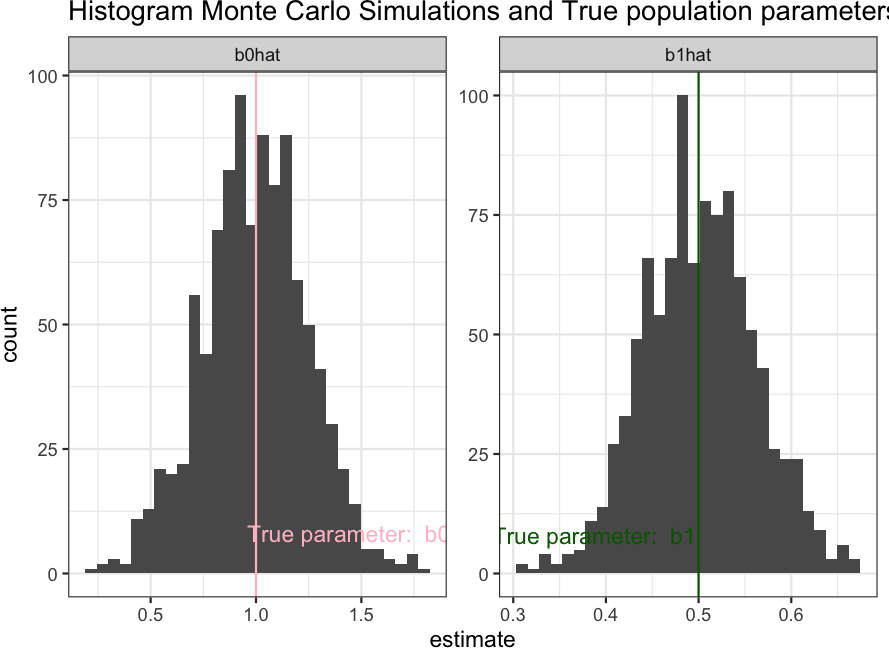
\includegraphics[width=0.8\linewidth]{MEM5220_R_files/figure-latex/fig8-1} 

}

\caption{Histogram b0 and b1 and true parameter}\label{fig:fig8}
\end{figure}

\begin{Shaded}
\begin{Highlighting}[]
\NormalTok{b1_sim <-}\StringTok{ }\NormalTok{MC_coef }\OperatorTok\StringTok{ }
\StringTok{  }\KeywordTok{filter}\NormalTok{(Simulated }\OperatorTok{==}\StringTok{ "b1"}\NormalTok{)}

\KeywordTok{mean}\NormalTok{(b1_sim}\OperatorTok{$}\NormalTok{estimate)}
\end{Highlighting}
\end{Shaded}

\begin{verbatim}
## [1] 0.5011414
\end{verbatim}

\begin{Shaded}
\begin{Highlighting}[]
\KeywordTok{var}\NormalTok{(b1_sim}\OperatorTok{$}\NormalTok{estimate) }\OperatorTok{==}\StringTok{ }\NormalTok{(}\KeywordTok{sd}\NormalTok{(b1_sim}\OperatorTok{$}\NormalTok{estimate))}\OperatorTok{^}\DecValTok{2}
\end{Highlighting}
\end{Shaded}

\begin{verbatim}
## [1] FALSE
\end{verbatim}

\begin{Shaded}
\begin{Highlighting}[]
\KeywordTok{all.equal}\NormalTok{(}\KeywordTok{var}\NormalTok{(b1_sim}\OperatorTok{$}\NormalTok{estimate) , (}\KeywordTok{sd}\NormalTok{(b1_sim}\OperatorTok{$}\NormalTok{estimate))}\OperatorTok{^}\DecValTok{2}\NormalTok{) }\CommentTok{# Floating point arithmetic!}
\end{Highlighting}
\end{Shaded}

\begin{verbatim}
## [1] TRUE
\end{verbatim}

\begin{Shaded}
\begin{Highlighting}[]
\KeywordTok{ggplot}\NormalTok{(}\DataTypeTok{data=}\NormalTok{ b1_sim, }\KeywordTok{aes}\NormalTok{(estimate)) }\OperatorTok{+}\StringTok{  }
\StringTok{  }\KeywordTok{geom_density}\NormalTok{(}\KeywordTok{aes}\NormalTok{(}\DataTypeTok{fill =}\NormalTok{ Simulated), }\DataTypeTok{alpha =} \FloatTok{0.2}\NormalTok{) }\OperatorTok{+}\StringTok{ }\CommentTok{# computes and draws the kernel density, which is the smoothed version of the histogram}
\StringTok{  }\CommentTok{# stat_function(fun = dnorm, args = list(mean = mean(b1_sim$estimate), sd = sd(b1_sim$estimate)), aes(colour = "true")) +}
\StringTok{  }\KeywordTok{stat_function}\NormalTok{(}\DataTypeTok{fun =}\NormalTok{ dnorm, }\DataTypeTok{args =} \KeywordTok{list}\NormalTok{(}\DataTypeTok{mean =} \FloatTok{0.5}\NormalTok{, }\DataTypeTok{sd =} \KeywordTok{sd}\NormalTok{(b1_sim}\OperatorTok{$}\NormalTok{estimate)), }\KeywordTok{aes}\NormalTok{(}\DataTypeTok{colour =} \StringTok{"true"}\NormalTok{)) }\OperatorTok{+}
\StringTok{  }\CommentTok{# labs(}
\StringTok{   }\CommentTok{#  title = "Kernel Density Monte Carlo Simulations vs. True population parameters"}
\StringTok{    }\CommentTok{# ) +}
\StringTok{  }\KeywordTok{scale_color_discrete}\NormalTok{(}\DataTypeTok{name=}\StringTok{""}\NormalTok{) }\OperatorTok{+}\StringTok{ }
\StringTok{  }\KeywordTok{theme_bw}\NormalTok{()}
\end{Highlighting}
\end{Shaded}

\begin{figure}

{\centering 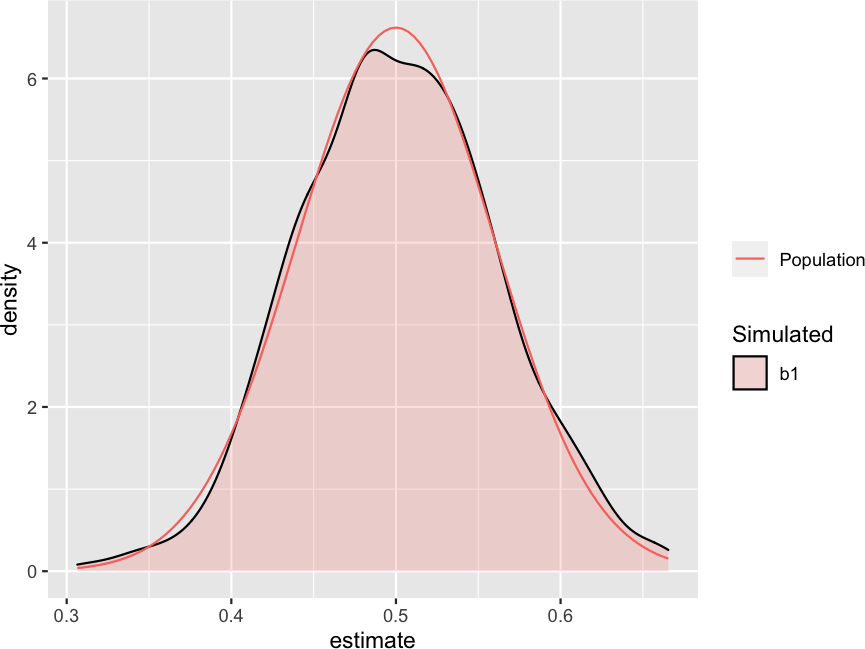
\includegraphics[width=0.8\linewidth]{MEM5220_R_files/figure-latex/fig9-1} 

}

\caption{Simulated and theoretical distributions of b1}\label{fig:fig9}
\end{figure}

\textbf{Rework this section} might have mixed up what is simulated and
what is biased

\hypertarget{violation-of-slr.4}{%
\paragraph{Violation of SLR.4}\label{violation-of-slr.4}}

To implement a violation of \textbf{SLR.4} (zero conditional mean)
consider a case where in the population \(u\) is not mean independent of
\(x\), for example

\[
\mathbf{E}(u|x) = \frac{x-4}{5}
\]

\begin{Shaded}
\begin{Highlighting}[]
\CommentTok{# Set the random seed}
\KeywordTok{set.seed}\NormalTok{(}\DecValTok{1234567}\NormalTok{)}

\CommentTok{# set sample size and number of simulations}
\NormalTok{n<-}\DecValTok{1000}\NormalTok{; r<-}\DecValTok{10000}

\CommentTok{# set true parameters: betas and sd of u}
\NormalTok{b0<-}\DecValTok{1}\NormalTok{; b1<-}\FloatTok{0.5}\NormalTok{; su<-}\DecValTok{2}

\CommentTok{# initialize b0hat and b1hat to store results later:}
\NormalTok{b0hat <-}\StringTok{ }\KeywordTok{numeric}\NormalTok{(r)}
\NormalTok{b1hat <-}\StringTok{ }\KeywordTok{numeric}\NormalTok{(r)}

\CommentTok{# Draw a sample of x, fixed over replications:}
\NormalTok{x <-}\StringTok{ }\KeywordTok{rnorm}\NormalTok{(n,}\DecValTok{4}\NormalTok{,}\DecValTok{1}\NormalTok{)}

\CommentTok{# repeat r times:}
\ControlFlowTok{for}\NormalTok{(j }\ControlFlowTok{in} \DecValTok{1}\OperatorTok{:}\NormalTok{r) \{}
\CommentTok{# Draw a sample of y:}
\NormalTok{u <-}\StringTok{ }\KeywordTok{rnorm}\NormalTok{(n, (x}\DecValTok{-4}\NormalTok{)}\OperatorTok{/}\DecValTok{5}\NormalTok{, su) }\CommentTok{# this is where manipulate the assumption of zero conditional mean}
\NormalTok{y <-}\StringTok{ }\NormalTok{b0 }\OperatorTok{+}\StringTok{ }\NormalTok{b1}\OperatorTok{*}\NormalTok{x }\OperatorTok{+}\StringTok{ }\NormalTok{u}

\CommentTok{# estimate parameters by OLS and store them in the vectors}
\NormalTok{bhat <-}\StringTok{ }\KeywordTok{coefficients}\NormalTok{( }\KeywordTok{lm}\NormalTok{(y}\OperatorTok{~}\NormalTok{x) )}
\NormalTok{b0hat[j] <-}\StringTok{ }\NormalTok{bhat[}\StringTok{"(Intercept)"}\NormalTok{]}
\NormalTok{b1hat[j] <-}\StringTok{ }\NormalTok{bhat[}\StringTok{"x"}\NormalTok{]}
\NormalTok{\}}
\end{Highlighting}
\end{Shaded}

OLS coefficients

\begin{Shaded}
\begin{Highlighting}[]
\CommentTok{# MC estimate of the expected values:}
\KeywordTok{mean}\NormalTok{(b0hat)}
\end{Highlighting}
\end{Shaded}

\begin{verbatim}
## [1] 0.1985388
\end{verbatim}

\begin{Shaded}
\begin{Highlighting}[]
\KeywordTok{mean}\NormalTok{(b1hat)}
\end{Highlighting}
\end{Shaded}

\begin{verbatim}
## [1] 0.7000466
\end{verbatim}

\begin{Shaded}
\begin{Highlighting}[]
\CommentTok{# MC estimate of the variances:}
\KeywordTok{var}\NormalTok{(b0hat)}
\end{Highlighting}
\end{Shaded}

\begin{verbatim}
## [1] 0.0690833
\end{verbatim}

\begin{Shaded}
\begin{Highlighting}[]
\KeywordTok{var}\NormalTok{(b1hat)}
\end{Highlighting}
\end{Shaded}

\begin{verbatim}
## [1] 0.004069063
\end{verbatim}

The average estimates are far from the population parameters
\(\beta_0=1\) and \(\beta_1 = 0.5\)!

\hypertarget{violation-of-slr.5}{%
\paragraph{Violation of SLR.5}\label{violation-of-slr.5}}

Homoskedasticity is not required for unbiasedness but for it is a
requirement for the theorem of sampling variance. Consider the following
heteroskedastic behavior of \(u\) given \(x\).

\begin{Shaded}
\begin{Highlighting}[]
\CommentTok{# Set the random seed}
\KeywordTok{set.seed}\NormalTok{(}\DecValTok{1234567}\NormalTok{)}

\CommentTok{# set sample size and number of simulations}
\NormalTok{n<-}\DecValTok{1000}\NormalTok{; r<-}\DecValTok{10000}

\CommentTok{# set true parameters: betas and sd of u}
\NormalTok{b0<-}\DecValTok{1}\NormalTok{; b1<-}\FloatTok{0.5}\NormalTok{; su<-}\DecValTok{2}

\CommentTok{# initialize b0hat and b1hat to store results later:}
\NormalTok{b0hat <-}\StringTok{ }\KeywordTok{numeric}\NormalTok{(r)}
\NormalTok{b1hat <-}\StringTok{ }\KeywordTok{numeric}\NormalTok{(r)}

\CommentTok{# Draw a sample of x, fixed over replications:}
\NormalTok{x <-}\StringTok{ }\KeywordTok{rnorm}\NormalTok{(n,}\DecValTok{4}\NormalTok{,}\DecValTok{1}\NormalTok{)}

\CommentTok{# repeat r times:}
\ControlFlowTok{for}\NormalTok{(j }\ControlFlowTok{in} \DecValTok{1}\OperatorTok{:}\NormalTok{r) \{}
  \CommentTok{# Draw a sample of y:}
\NormalTok{  varu <-}\StringTok{ }\DecValTok{4}\OperatorTok{/}\KeywordTok{exp}\NormalTok{(}\FloatTok{4.5}\NormalTok{) }\OperatorTok{*}\StringTok{ }\KeywordTok{exp}\NormalTok{(x)}
\NormalTok{  u <-}\StringTok{ }\KeywordTok{rnorm}\NormalTok{(n, }\DecValTok{0}\NormalTok{, }\KeywordTok{sqrt}\NormalTok{(varu) )}
\NormalTok{  y <-}\StringTok{ }\NormalTok{b0 }\OperatorTok{+}\StringTok{ }\NormalTok{b1}\OperatorTok{*}\NormalTok{x }\OperatorTok{+}\StringTok{ }\NormalTok{u}
  
  \CommentTok{# estimate parameters by OLS and store them in the vectors}
\NormalTok{  lm_heterosced <-}\StringTok{ }\KeywordTok{lm}\NormalTok{(y}\OperatorTok{~}\NormalTok{x)}
  
\NormalTok{  bhat <-}\StringTok{ }\KeywordTok{coefficients}\NormalTok{( }\KeywordTok{lm}\NormalTok{(y}\OperatorTok{~}\NormalTok{x) )}
\NormalTok{  b0hat[j] <-}\StringTok{ }\NormalTok{bhat[}\StringTok{"(Intercept)"}\NormalTok{]}
\NormalTok{  b1hat[j] <-}\StringTok{ }\NormalTok{bhat[}\StringTok{"x"}\NormalTok{]}
\NormalTok{\}}
\end{Highlighting}
\end{Shaded}

\begin{Shaded}
\begin{Highlighting}[]
\KeywordTok{summary}\NormalTok{(lm_heterosced) }\CommentTok{# just the last sample of the MC-simulation}
\end{Highlighting}
\end{Shaded}

\begin{verbatim}
## 
## Call:
## lm(formula = y ~ x)
## 
## Residuals:
##      Min       1Q   Median       3Q      Max 
## -23.6742  -0.9033   0.0052   1.0012   9.3411 
## 
## Coefficients:
##             Estimate Std. Error t value Pr(>|t|)    
## (Intercept)  1.24088    0.27158   4.569 5.51e-06 ***
## x            0.44561    0.06593   6.759 2.37e-11 ***
## ---
## Signif. codes:  0 '***' 0.001 '**' 0.01 '*' 0.05 '.' 0.1 ' ' 1
## 
## Residual standard error: 2.075 on 998 degrees of freedom
## Multiple R-squared:  0.04377,    Adjusted R-squared:  0.04281 
## F-statistic: 45.68 on 1 and 998 DF,  p-value: 2.367e-11
\end{verbatim}

Plot the residual against the regressor suspected of creating
heteroskedasticity, or more generally, the fitted values of the
regression.

\begin{Shaded}
\begin{Highlighting}[]
\NormalTok{res <-}\StringTok{ }\KeywordTok{residuals}\NormalTok{(lm_heterosced)}
\NormalTok{yhat <-}\StringTok{ }\KeywordTok{fitted}\NormalTok{(lm_heterosced)}
\end{Highlighting}
\end{Shaded}

\begin{Shaded}
\begin{Highlighting}[]
\KeywordTok{par}\NormalTok{(}\DataTypeTok{mfrow =} \KeywordTok{c}\NormalTok{(}\DecValTok{1}\NormalTok{,}\DecValTok{2}\NormalTok{))}
\KeywordTok{plot}\NormalTok{(x, res, }\DataTypeTok{ylab =} \StringTok{"residuals"}\NormalTok{)}
\KeywordTok{plot}\NormalTok{(yhat, res, }\DataTypeTok{xlab =} \StringTok{"fitted values"}\NormalTok{, }\DataTypeTok{ylab =} \StringTok{"residuals"}\NormalTok{)}
\end{Highlighting}
\end{Shaded}

\begin{figure}

{\centering 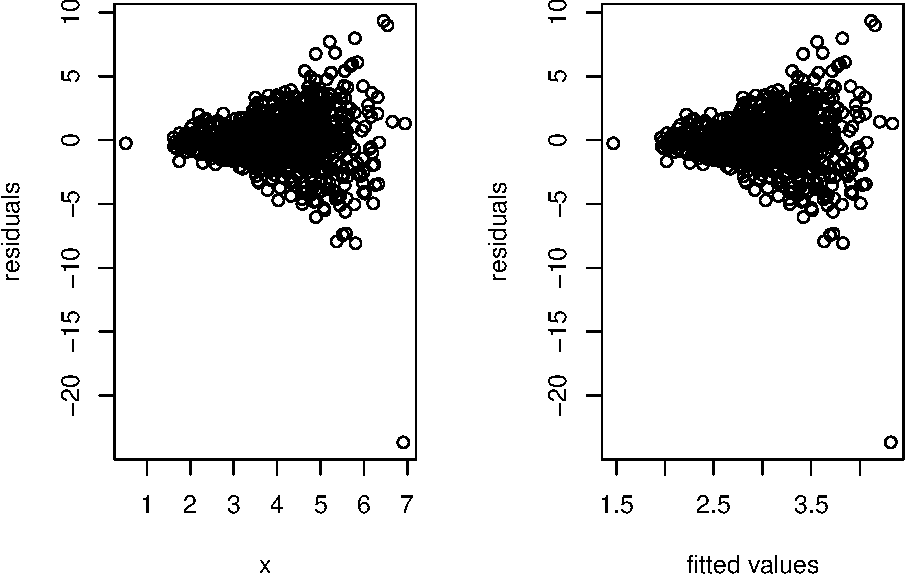
\includegraphics[width=0.8\linewidth]{MEM5220_R_files/figure-latex/fig10-1} 

}

\caption{Heteroskedasticity in the simulated data}\label{fig:fig10}
\end{figure}

\begin{Shaded}
\begin{Highlighting}[]
\CommentTok{# MC estimate of the expected values:}
\KeywordTok{mean}\NormalTok{(b0hat)}
\end{Highlighting}
\end{Shaded}

\begin{verbatim}
## [1] 1.0019
\end{verbatim}

\begin{Shaded}
\begin{Highlighting}[]
\KeywordTok{mean}\NormalTok{(b1hat)}
\end{Highlighting}
\end{Shaded}

\begin{verbatim}
## [1] 0.4992376
\end{verbatim}

\begin{Shaded}
\begin{Highlighting}[]
\CommentTok{# MC estimate of the variances:}
\KeywordTok{var}\NormalTok{(b0hat)}
\end{Highlighting}
\end{Shaded}

\begin{verbatim}
## [1] 0.08967037
\end{verbatim}

\begin{Shaded}
\begin{Highlighting}[]
\KeywordTok{var}\NormalTok{(b1hat)}
\end{Highlighting}
\end{Shaded}

\begin{verbatim}
## [1] 0.007264373
\end{verbatim}

Unbiasedness is provided but sampling variance is incorrect (compared to
the results provided above).

\hypertarget{nonlinearities}{%
\subsection{Nonlinearities}\label{nonlinearities}}

Sometimes the scatter plot diagram or some theoretical considerations
suggest a non-linear relationship. The most popular non-linear
relationships involve logarithms of the dependent or independent
variables and polynomial functions.

We will use a new dataset, \emph{wage1}, for this section. A detailed
exploratory analysis of the dataset is left to the reader.

\begin{Shaded}
\begin{Highlighting}[]
\KeywordTok{data}\NormalTok{(}\StringTok{"wage1"}\NormalTok{)}
\KeywordTok{attach}\NormalTok{(wage1)}
\end{Highlighting}
\end{Shaded}

\begin{verbatim}
## The following objects are masked from wage1 (pos = 5):
## 
##     clerocc, construc, educ, exper, expersq, female, lwage,
##     married, ndurman, nonwhite, northcen, numdep, profocc,
##     profserv, services, servocc, smsa, south, tenure, tenursq,
##     trade, trcommpu, wage, west
\end{verbatim}

\hypertarget{predicated-variable-transformation}{%
\subsubsection{Predicated variable
transformation}\label{predicated-variable-transformation}}

A common variance stabilizing transformation (VST) when we see
increasing variance in a fitted versus residuals plot is \(log(Y)\).

Related, to use the \emph{log} of an independent variable is to make its
distribution closer to the normal distribution.

\begin{Shaded}
\begin{Highlighting}[]
\CommentTok{# wage1$logwage <- log(wage1$wage) # one could also create a new variable }

\NormalTok{p1_wagehisto <-}\StringTok{ }\KeywordTok{ggplot}\NormalTok{(wage1)  }\OperatorTok{+}
\StringTok{  }\KeywordTok{geom_histogram}\NormalTok{(}\KeywordTok{aes}\NormalTok{(}\DataTypeTok{x =}\NormalTok{ wage), }\DataTypeTok{fill =} \StringTok{"red"}\NormalTok{, }\DataTypeTok{alpha =} \FloatTok{0.6}\NormalTok{) }\OperatorTok{+}
\StringTok{  }\KeywordTok{theme_bw}\NormalTok{()}


\NormalTok{p2_wagehisto <-}\StringTok{ }\KeywordTok{ggplot}\NormalTok{(wage1)  }\OperatorTok{+}
\StringTok{  }\KeywordTok{geom_histogram}\NormalTok{(}\KeywordTok{aes}\NormalTok{(}\DataTypeTok{x =}\NormalTok{ wage),  }\DataTypeTok{fill =} \StringTok{"blue"}\NormalTok{, }\DataTypeTok{alpha =} \FloatTok{0.6}\NormalTok{) }\OperatorTok{+}
\StringTok{  }\KeywordTok{scale_x_continuous}\NormalTok{(}\DataTypeTok{trans=}\StringTok{'log2'}\NormalTok{, }\StringTok{"Log Wage"}\NormalTok{) }\OperatorTok{+}\StringTok{ }\CommentTok{# instead of creating a new variable with simply define that the x-scale undergoes a logarithmic transformation}
\StringTok{  }\KeywordTok{theme_bw}\NormalTok{()}
\end{Highlighting}
\end{Shaded}

\begin{Shaded}
\begin{Highlighting}[]
\KeywordTok{ggarrange}\NormalTok{(p1_wagehisto, p2_wagehisto,  }
          \DataTypeTok{labels =} \KeywordTok{c}\NormalTok{(}\StringTok{"A"}\NormalTok{, }\StringTok{"B"}\NormalTok{),}
          \DataTypeTok{ncol =} \DecValTok{2}\NormalTok{, }\DataTypeTok{nrow =} \DecValTok{1}\NormalTok{)}
\end{Highlighting}
\end{Shaded}

\begin{verbatim}
## `stat_bin()` using `bins = 30`. Pick better value with `binwidth`.
## `stat_bin()` using `bins = 30`. Pick better value with `binwidth`.
\end{verbatim}

\begin{figure}

{\centering 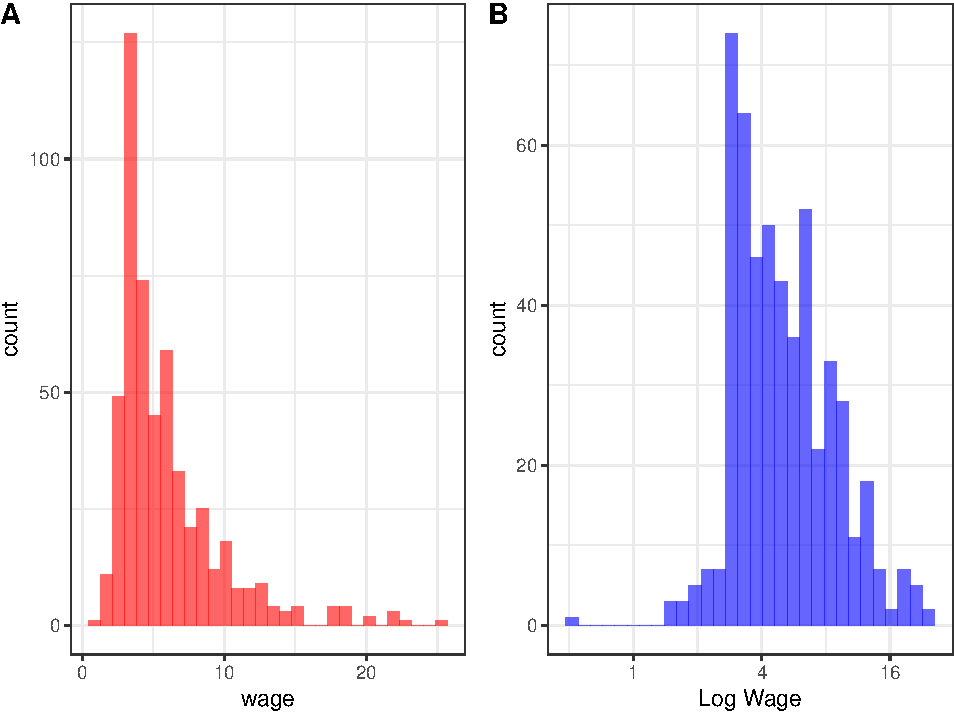
\includegraphics[width=0.8\linewidth]{MEM5220_R_files/figure-latex/fig11-1} 

}

\caption{Histogram of wage and log(wage)}\label{fig:fig11}
\end{figure}

A model with a log transformed response:

\begin{equation}
log(Y_{i}) = \beta_{0} + \beta_{1} \times x_{i} + \epsilon_{i}
\end{equation}

\begin{Shaded}
\begin{Highlighting}[]
\NormalTok{lm_wage <-}\StringTok{ }\KeywordTok{lm}\NormalTok{(wage }\OperatorTok{~}\StringTok{ }\NormalTok{educ, }\DataTypeTok{data =}\NormalTok{ wage1)}
\NormalTok{lm_wage1 <-}\StringTok{ }\KeywordTok{lm}\NormalTok{(}\KeywordTok{log}\NormalTok{(wage)}\OperatorTok{~}\StringTok{ }\NormalTok{educ, }\DataTypeTok{data =}\NormalTok{  wage1)}
\KeywordTok{summary}\NormalTok{(lm_wage)}
\end{Highlighting}
\end{Shaded}

\begin{verbatim}
## 
## Call:
## lm(formula = wage ~ educ, data = wage1)
## 
## Residuals:
##     Min      1Q  Median      3Q     Max 
## -5.3396 -2.1501 -0.9674  1.1921 16.6085 
## 
## Coefficients:
##             Estimate Std. Error t value Pr(>|t|)    
## (Intercept) -0.90485    0.68497  -1.321    0.187    
## educ         0.54136    0.05325  10.167   <2e-16 ***
## ---
## Signif. codes:  0 '***' 0.001 '**' 0.01 '*' 0.05 '.' 0.1 ' ' 1
## 
## Residual standard error: 3.378 on 524 degrees of freedom
## Multiple R-squared:  0.1648, Adjusted R-squared:  0.1632 
## F-statistic: 103.4 on 1 and 524 DF,  p-value: < 2.2e-16
\end{verbatim}

\begin{Shaded}
\begin{Highlighting}[]
\KeywordTok{summary}\NormalTok{(lm_wage1)}
\end{Highlighting}
\end{Shaded}

\begin{verbatim}
## 
## Call:
## lm(formula = log(wage) ~ educ, data = wage1)
## 
## Residuals:
##      Min       1Q   Median       3Q      Max 
## -2.21158 -0.36393 -0.07263  0.29712  1.52339 
## 
## Coefficients:
##             Estimate Std. Error t value Pr(>|t|)    
## (Intercept) 0.583773   0.097336   5.998 3.74e-09 ***
## educ        0.082744   0.007567  10.935  < 2e-16 ***
## ---
## Signif. codes:  0 '***' 0.001 '**' 0.01 '*' 0.05 '.' 0.1 ' ' 1
## 
## Residual standard error: 0.4801 on 524 degrees of freedom
## Multiple R-squared:  0.1858, Adjusted R-squared:  0.1843 
## F-statistic: 119.6 on 1 and 524 DF,  p-value: < 2.2e-16
\end{verbatim}

Plotting Diagnostics for Linear Models

\begin{Shaded}
\begin{Highlighting}[]
\KeywordTok{plot}\NormalTok{(lm_wage)}
\end{Highlighting}
\end{Shaded}

\begin{figure}

{\centering 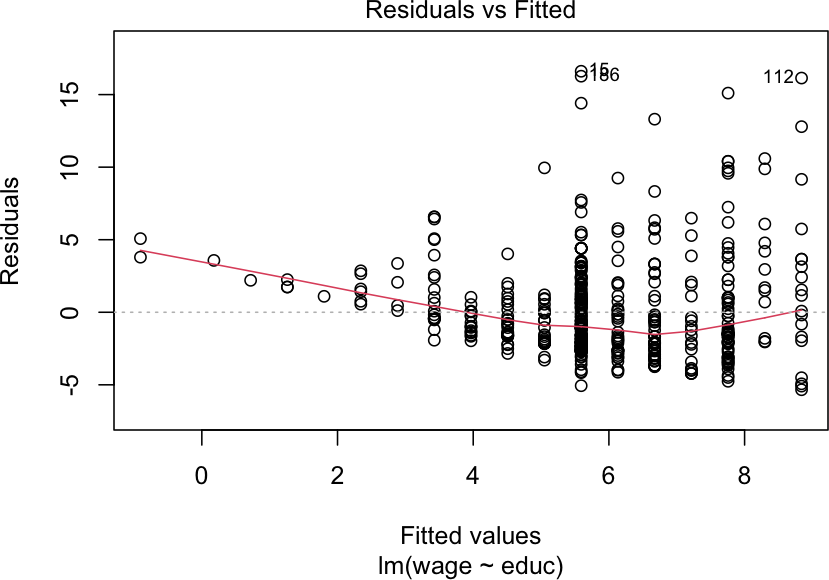
\includegraphics[width=0.8\linewidth]{MEM5220_R_files/figure-latex/fig12-1} 

}

\caption{Regression diagnostics plot base R - Linear Relationship}\label{fig:fig121}
\end{figure}
\begin{figure}

{\centering 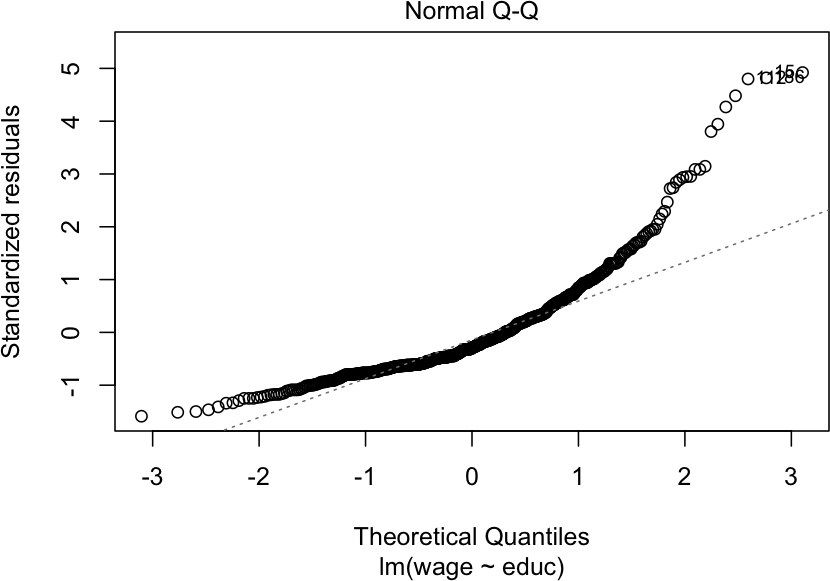
\includegraphics[width=0.8\linewidth]{MEM5220_R_files/figure-latex/fig12-2} 

}

\caption{Regression diagnostics plot base R - Linear Relationship}\label{fig:fig122}
\end{figure}
\begin{figure}

{\centering 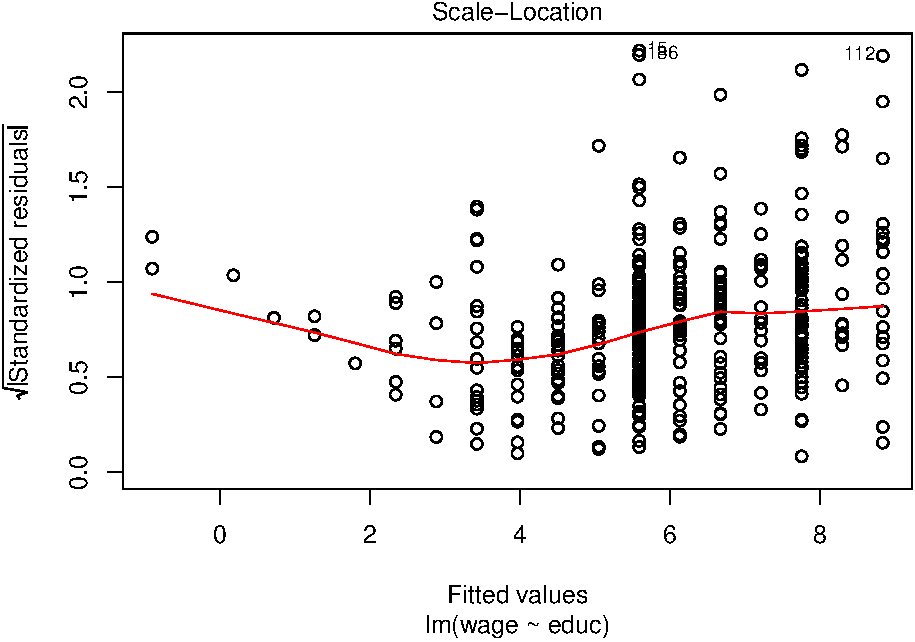
\includegraphics[width=0.8\linewidth]{MEM5220_R_files/figure-latex/fig12-3} 

}

\caption{Regression diagnostics plot base R - Linear Relationship}\label{fig:fig123}
\end{figure}
\begin{figure}

{\centering 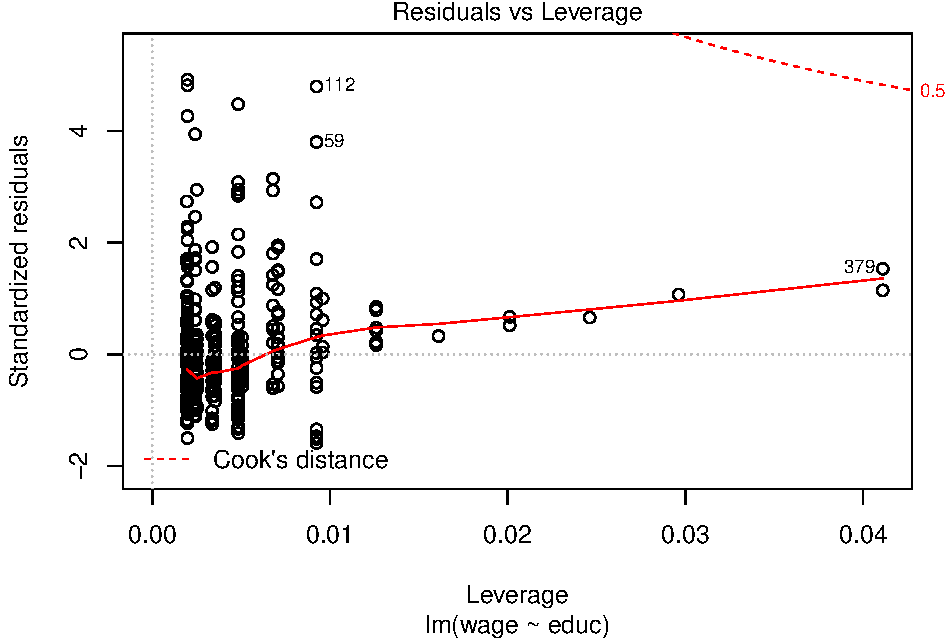
\includegraphics[width=0.8\linewidth]{MEM5220_R_files/figure-latex/fig12-4} 

}

\caption{Regression diagnostics plot base R - Linear Relationship}\label{fig:fig124}
\end{figure}

\begin{Shaded}
\begin{Highlighting}[]
\KeywordTok{autoplot}\NormalTok{(lm_wage, }\DataTypeTok{which =} \DecValTok{1}\OperatorTok{:}\DecValTok{6}\NormalTok{, }\DataTypeTok{colour =} \StringTok{'dodgerblue3'}\NormalTok{,}
         \DataTypeTok{smooth.colour =} \StringTok{'red'}\NormalTok{, }\DataTypeTok{smooth.linetype =} \StringTok{'dashed'}\NormalTok{,}
         \DataTypeTok{ad.colour =} \StringTok{'blue'}\NormalTok{,}
         \DataTypeTok{label =} \OtherTok{FALSE}\NormalTok{,}
         \DataTypeTok{label.size =} \DecValTok{3}\NormalTok{, }\DataTypeTok{label.n =} \DecValTok{5}\NormalTok{, }\DataTypeTok{label.colour =} \StringTok{'blue'}\NormalTok{,}
         \DataTypeTok{ncol =} \DecValTok{3}\NormalTok{) }\OperatorTok{+}
\StringTok{  }\KeywordTok{theme_bw}\NormalTok{()}
\end{Highlighting}
\end{Shaded}

\begin{figure}

{\centering 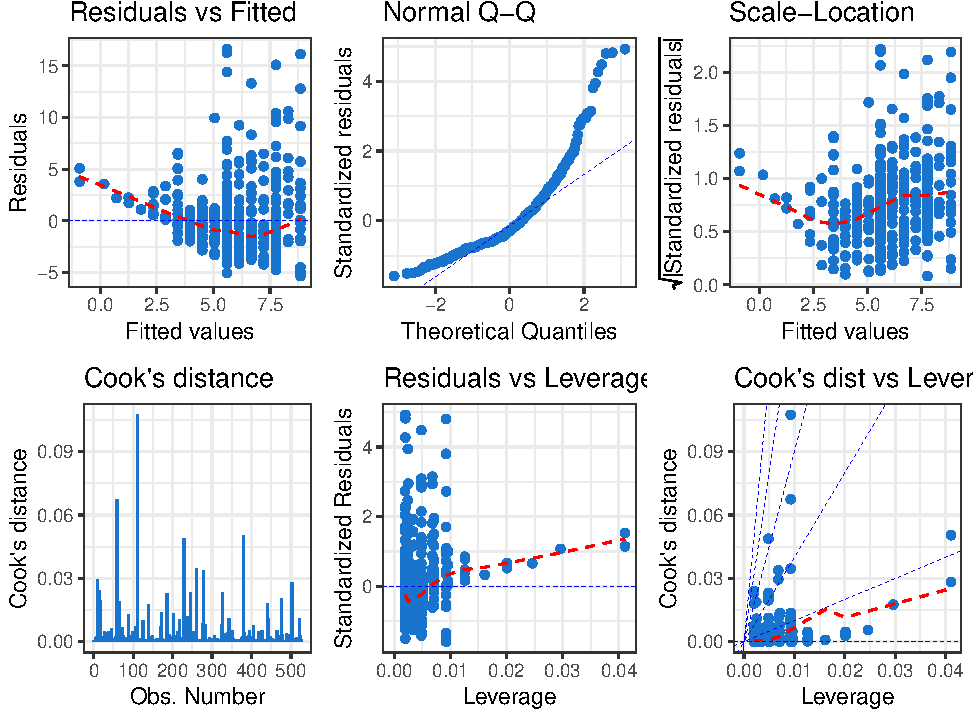
\includegraphics[width=0.8\linewidth]{MEM5220_R_files/figure-latex/fig13-1} 

}

\caption{Regression diagnostics autoplot(ggplot) - Linear Relationship}\label{fig:fig13}
\end{figure}

\begin{Shaded}
\begin{Highlighting}[]
\KeywordTok{autoplot}\NormalTok{(lm_wage1, }\DataTypeTok{which =} \DecValTok{1}\OperatorTok{:}\DecValTok{6}\NormalTok{, }\DataTypeTok{colour =} \StringTok{'dodgerblue3'}\NormalTok{,}
         \DataTypeTok{smooth.colour =} \StringTok{'red'}\NormalTok{, }\DataTypeTok{smooth.linetype =} \StringTok{'dashed'}\NormalTok{,}
         \DataTypeTok{ad.colour =} \StringTok{'blue'}\NormalTok{,}
         \DataTypeTok{label =} \OtherTok{FALSE}\NormalTok{,}
         \DataTypeTok{label.size =} \DecValTok{3}\NormalTok{, }\DataTypeTok{label.n =} \DecValTok{5}\NormalTok{, }\DataTypeTok{label.colour =} \StringTok{'blue'}\NormalTok{,}
         \DataTypeTok{ncol =} \DecValTok{3}\NormalTok{) }\OperatorTok{+}
\StringTok{  }\KeywordTok{theme_bw}\NormalTok{()}
\end{Highlighting}
\end{Shaded}

\begin{figure}

{\centering 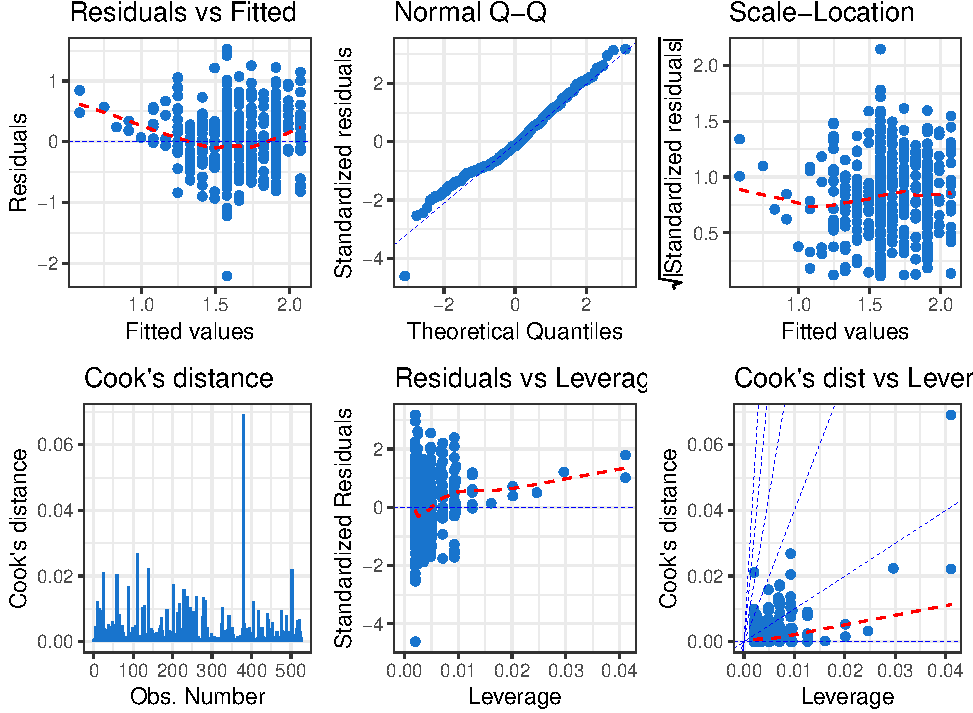
\includegraphics[width=0.8\linewidth]{MEM5220_R_files/figure-latex/fig14-1} 

}

\caption{Regression diagnostics - Non-Linear Relationship}\label{fig:fig14}
\end{figure}

\begin{Shaded}
\begin{Highlighting}[]
\NormalTok{p1_nonlinearities <-}\StringTok{ }\KeywordTok{ggplot}\NormalTok{(wage1, }\KeywordTok{aes}\NormalTok{(}\DataTypeTok{x =}\NormalTok{ educ, }\DataTypeTok{y =}\NormalTok{ wage )) }\OperatorTok{+}
\StringTok{  }\KeywordTok{geom_point}\NormalTok{()   }\OperatorTok{+}\StringTok{ }
\StringTok{  }\KeywordTok{scale_y_continuous}\NormalTok{(}\DataTypeTok{trans=}\StringTok{'log2'}\NormalTok{, }\StringTok{"Log Wage"}\NormalTok{) }\OperatorTok{+}\StringTok{ }
\StringTok{  }\KeywordTok{stat_smooth}\NormalTok{(}\KeywordTok{aes}\NormalTok{(}\DataTypeTok{fill=}\StringTok{"Linear Model"}\NormalTok{),}\DataTypeTok{size=}\DecValTok{1}\NormalTok{,}\DataTypeTok{method =} \StringTok{"lm"}\NormalTok{ ,}\DataTypeTok{span =}\FloatTok{0.3}\NormalTok{, }\DataTypeTok{se=}\NormalTok{F) }\OperatorTok{+}\StringTok{ }
\StringTok{  }\KeywordTok{guides}\NormalTok{(}\DataTypeTok{fill =} \KeywordTok{guide_legend}\NormalTok{(}\StringTok{"Model Type"}\NormalTok{)) }\OperatorTok{+}\StringTok{ }
\StringTok{  }\KeywordTok{theme_bw}\NormalTok{()}
\end{Highlighting}
\end{Shaded}

Note that if we re-scale the model from a log scale back to the original
scale of the data, we now have

\begin{equation}
Y_{i} = exp(\beta_{0} + \beta_{1} \times x_{i})  \times exp(\epsilon_{i})
\end{equation}

which has errors entering in a multiplicative fashion.

\begin{Shaded}
\begin{Highlighting}[]
\NormalTok{log.model.df <-}\StringTok{ }\KeywordTok{data.frame}\NormalTok{(}\DataTypeTok{x =}\NormalTok{ wage1}\OperatorTok{$}\NormalTok{educ,}
                           \DataTypeTok{y =} \KeywordTok{exp}\NormalTok{(}\KeywordTok{fitted}\NormalTok{(lm_wage1))) }\CommentTok{# This is essentially exp(b0_wage1 + b1_wage1 * wage1$educ) }
\end{Highlighting}
\end{Shaded}

\begin{Shaded}
\begin{Highlighting}[]
\NormalTok{p2_nonlinearities <-}\StringTok{ }\KeywordTok{ggplot}\NormalTok{(wage1, }\KeywordTok{aes}\NormalTok{(}\DataTypeTok{x =}\NormalTok{ educ, }\DataTypeTok{y =}\NormalTok{ wage))  }\OperatorTok{+}
\StringTok{  }\KeywordTok{geom_point}\NormalTok{()   }\OperatorTok{+}
\StringTok{  }\KeywordTok{geom_line}\NormalTok{(}\DataTypeTok{data =}\NormalTok{ log.model.df, }\KeywordTok{aes}\NormalTok{(x, y, }\DataTypeTok{color =} \StringTok{"Log Model"}\NormalTok{), }\DataTypeTok{size =} \DecValTok{1}\NormalTok{, }\DataTypeTok{linetype =} \DecValTok{2}\NormalTok{)  }\OperatorTok{+}
\StringTok{  }\KeywordTok{guides}\NormalTok{(}\DataTypeTok{color =} \KeywordTok{guide_legend}\NormalTok{(}\StringTok{"Model Type"}\NormalTok{)) }\OperatorTok{+}\StringTok{ }
\StringTok{  }\KeywordTok{theme_bw}\NormalTok{()}
\end{Highlighting}
\end{Shaded}

\begin{Shaded}
\begin{Highlighting}[]
\KeywordTok{ggarrange}\NormalTok{(p1_nonlinearities, p2_nonlinearities,  }
          \DataTypeTok{labels =} \KeywordTok{c}\NormalTok{(}\StringTok{"A"}\NormalTok{, }\StringTok{"B"}\NormalTok{),}
          \DataTypeTok{ncol =} \DecValTok{2}\NormalTok{, }\DataTypeTok{nrow =} \DecValTok{1}\NormalTok{)}
\end{Highlighting}
\end{Shaded}

\begin{figure}

{\centering 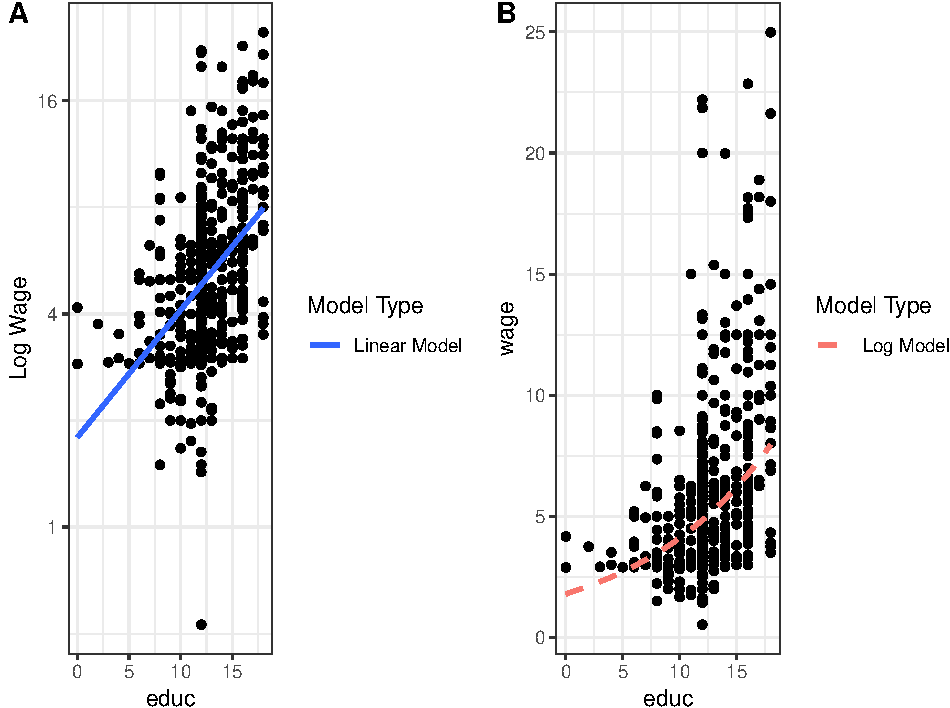
\includegraphics[width=0.8\linewidth]{MEM5220_R_files/figure-latex/fig15-1} 

}

\caption{Wages by Education - Different transformations}\label{fig:fig15}
\end{figure}

A: Plotting the data on the transformed log scale and adding the fitted
line, the relationship again appears linear, and the variation about the
fitted line looks more constant.

B: By plotting the data on the original scale, and adding the fitted
regression, we see an exponential relationship. However, this is still a
\emph{linear} model, since the new transformed response, \(log(Y_{i}\),
is still a \emph{linear} combination of the predictors. In other words,
only \(\beta\) needs to be linear, not the \(x\) values.

\emph{NOTE:}

The example comes from the Wooldrige book but the variable educ looks
more like count data. A Poisson GLM might seems like a better choice.

\textbf{Quadratic Model}

\begin{equation}
Y_{i} = \beta_{0} + \beta_{1} \times x^2_{i})  \times \epsilon_{i}
\end{equation}

New dataset from Wooldrige: Collected from the real estate pages of the
Boston Globe during 1990. These are homes that sold in the Boston, MA
area.

\begin{Shaded}
\begin{Highlighting}[]
\KeywordTok{data}\NormalTok{(}\StringTok{"hprice1"}\NormalTok{)}
\KeywordTok{attach}\NormalTok{(hprice1)}
\end{Highlighting}
\end{Shaded}

\begin{verbatim}
## The following objects are masked from hprice1 (pos = 5):
## 
##     assess, bdrms, colonial, lassess, llotsize, lotsize, lprice,
##     lsqrft, price, sqrft
\end{verbatim}

In R, independent variables involving mathematical operators can be
included in regression equation with the function \texttt{I()}

\begin{Shaded}
\begin{Highlighting}[]
\NormalTok{lm_hprice <-}\StringTok{ }\KeywordTok{lm}\NormalTok{(price }\OperatorTok{~}\StringTok{ }\NormalTok{sqrft, }\DataTypeTok{data  =}\NormalTok{ hprice1)}
\NormalTok{lm_hprice1 <-}\StringTok{ }\KeywordTok{lm}\NormalTok{(price }\OperatorTok{~}\StringTok{ }\NormalTok{sqrft }\OperatorTok{+}\StringTok{ }\KeywordTok{I}\NormalTok{(sqrft}\OperatorTok{^}\DecValTok{2}\NormalTok{), }\DataTypeTok{data  =}\NormalTok{ hprice1)}
\end{Highlighting}
\end{Shaded}

Alternatively use the \texttt{poly()} function. Be careful of the
additional argument \texttt{raw}.

\begin{Shaded}
\begin{Highlighting}[]
\NormalTok{lm_hprice2 <-}\StringTok{ }\KeywordTok{lm}\NormalTok{(price }\OperatorTok{~}\StringTok{ }\KeywordTok{poly}\NormalTok{(sqrft, }\DataTypeTok{degree =} \DecValTok{2}\NormalTok{),  }\DataTypeTok{data  =}\NormalTok{ hprice1) }
\NormalTok{lm_hprice3 <-}\StringTok{ }\KeywordTok{lm}\NormalTok{(price }\OperatorTok{~}\StringTok{ }\KeywordTok{poly}\NormalTok{(sqrft, }\DataTypeTok{degree =} \DecValTok{2}\NormalTok{, }\DataTypeTok{raw =} \OtherTok{TRUE}\NormalTok{),  }\DataTypeTok{data  =}\NormalTok{ hprice1) }\CommentTok{# if true, use raw and not orthogonal polynomials.}
\end{Highlighting}
\end{Shaded}

\begin{Shaded}
\begin{Highlighting}[]
\KeywordTok{unname}\NormalTok{(}\KeywordTok{coef}\NormalTok{(lm_hprice1))}
\end{Highlighting}
\end{Shaded}

\begin{verbatim}
## [1]  1.849453e+02 -1.710855e-02  3.262809e-05
\end{verbatim}

\begin{Shaded}
\begin{Highlighting}[]
\KeywordTok{unname}\NormalTok{(}\KeywordTok{coef}\NormalTok{(lm_hprice2))}
\end{Highlighting}
\end{Shaded}

\begin{verbatim}
## [1] 293.5460 754.8517 135.6051
\end{verbatim}

\begin{Shaded}
\begin{Highlighting}[]
\KeywordTok{unname}\NormalTok{(}\KeywordTok{coef}\NormalTok{(lm_hprice3))}
\end{Highlighting}
\end{Shaded}

\begin{verbatim}
## [1]  1.849453e+02 -1.710855e-02  3.262809e-05
\end{verbatim}

\begin{Shaded}
\begin{Highlighting}[]
\KeywordTok{all.equal}\NormalTok{(}\KeywordTok{unname}\NormalTok{(}\KeywordTok{coef}\NormalTok{(lm_hprice1)), }\KeywordTok{unname}\NormalTok{(}\KeywordTok{coef}\NormalTok{(lm_hprice2)))}
\end{Highlighting}
\end{Shaded}

\begin{verbatim}
## [1] "Mean relative difference: 5.401501"
\end{verbatim}

\begin{Shaded}
\begin{Highlighting}[]
\KeywordTok{all.equal}\NormalTok{(}\KeywordTok{unname}\NormalTok{(}\KeywordTok{coef}\NormalTok{(lm_hprice1)), }\KeywordTok{unname}\NormalTok{(}\KeywordTok{coef}\NormalTok{(lm_hprice3)))}
\end{Highlighting}
\end{Shaded}

\begin{verbatim}
## [1] TRUE
\end{verbatim}

\begin{Shaded}
\begin{Highlighting}[]
\KeywordTok{all.equal}\NormalTok{(}\KeywordTok{fitted}\NormalTok{(lm_hprice1), }\KeywordTok{fitted}\NormalTok{(lm_hprice2))}
\end{Highlighting}
\end{Shaded}

\begin{verbatim}
## [1] TRUE
\end{verbatim}

\begin{Shaded}
\begin{Highlighting}[]
\KeywordTok{all.equal}\NormalTok{(}\KeywordTok{fitted}\NormalTok{(lm_hprice1), }\KeywordTok{fitted}\NormalTok{(lm_hprice3))}
\end{Highlighting}
\end{Shaded}

\begin{verbatim}
## [1] TRUE
\end{verbatim}

\hypertarget{inference-for-simple-linear-regression}{%
\subsection{Inference for Simple Linear
Regression}\label{inference-for-simple-linear-regression}}

\begin{quote}
``There are three types of lies: lies, damn lies, and statistics''
\emph{Benjamin Disraeli}
\end{quote}

\hypertarget{multiple-linear-regression}{%
\section{Multiple Linear Regression}\label{multiple-linear-regression}}

\begin{center}\rule{0.5\linewidth}{\linethickness}\end{center}

\textbf{Note}

A \textbf{(general) linear model} is similar to the simple variant, but
with a multivariate \(x \epsilon \!R^{\rho}\) and a mean given by a
hyperplane in place of a single line.

\begin{itemize}
\tightlist
\item
  General principles are the same as the simple case
\item
  Math is more difficult because we need to use matrices
\item
  Interpretation is more difficult because the \(\beta_{j}\) are effects
  conditional on the other variables
\end{itemize}

Many would retain the same signs as the simple linear regression, but
the magnitudes would be smaller. In some cases, it is possible for the
relationship to flip directions when a second (highly correlated)
variable is added.

\begin{center}\rule{0.5\linewidth}{\linethickness}\end{center}

The file was creating using \texttt{R} version \texttt{3.5.1}.

\hypertarget{binarymodels}{%
\chapter{Binary limited dependent variable models}\label{binarymodels}}

In this section we discuss probit and logit models

\bibliography{MEM5220.bib,packages.bib}


\end{document}
